\documentclass[msc,cogsci]{infthesis/infthesis}
\title{Rhythmic structure in performed Jazz music}
\author{Bastiaan van der Weij}

\usepackage[round]{natbib}
\usepackage{graphicx}
\usepackage{subfig}
\usepackage{epstopdf}
\usepackage{amsmath}
\usepackage{qtree}
\usepackage{algorithm}
\usepackage{algpseudocode}
\usepackage{array}


%\date{Augustus 17, 2012}

% Figures to generate:
% Likely and unlikely interpretations of a rhythm
% Examples of how combination and subdivision analysis works
% Example of ambiguity
% Example of too fine-grained analysis and too coarse
% Example of tree translated to notes at different levels
% Example of swung notes
% Phase shifted rhythm for illustrating importance of prior
% Syncopation to illustrate prior, perhaps using Temperley's examples

\abstract{%
   
}

\begin{document}


\begin{preliminary}
\maketitle
%% Acknowledgements
\begin{acknowledgements}

\end{acknowledgements}

%% Next we need to have the declaration.
\standarddeclaration

%% Finally, a dedication (this is optional -- uncomment the following line if
%% you want one).
% \dedication{To my mummy.}

%% Create the table of contents
\tableofcontents

%% If you want a list of figures or tables, uncomment the appropriate line(s)
% \listoffigures
% \listoftables

\end{preliminary}

%%%%%%%%
%% Include your chapter files here. See the sample chapter file for the basic
%% format.

%\abstract{%
   
}
%\chapter{Introduction}
\label{sec:introduction}

The work in this thesis is concerned with the analysis of the rhythmic structure in performances of music. We will study rhythmic structure in isolation of other structures that may be present in the music like melody or harmony.

This chapter will introduce concepts used throughout this thesis and discuss related studies. First, rhythmic structure is introduced. Then in section \ref{sec:performances}, structure will be related to performance and finally in section \ref{sec:introducing} the approach presented in this thesis will be introduced.

The rest of this thesis is structured as follows: In chapter \ref{sec:method}, our approach will be described in detail. Chapter \ref{sec:method} will also introduce the annotated jazz corpus that was produced for this thesis. In chapter \ref{sec:evaluation}, we will describe how we intent to evaluate our system. Then in chapter \ref{sec:results} the system will be evaluated on the jazz corpus. Chapter \ref{sec:discussion} will discuss to what extent the system was successful based on the results and improvements will be suggested. Finally, chapter \ref{sec:conclusion} will present the conclusions of this thesis.

\section{Rhythmic Structure}
\label{sec:structure}

A rhythm, in most Western music traditions, is composed of metrical units, rests or notes, whose duration is specified relative to each other. A note tells the performer to play some pitch for the duration of the note, a rest indicates a silence for the duration of the rest. Durations are specified as subdivisions of the duration of a whole note: some common subdivisions are: half notes or rests, quarter notes or rests, eighth notes or rests, etcetera. Their notation in the so-called staff music notation is illustrated in table \ref{tab:notation}. Apart from the duple divisions mentioned above, triple divisions, quintuple and any other prime number divisions are allowed as well although divisions higher than triple are rare. 

\begin{table}
\caption{Some music notation conventions.}
\label{tab:notation}
\centering
\begin{tabular}{lllll}
\parbox{0.15\linewidth}{
\centering
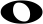
\includegraphics[scale=0.5]{img/whole_note}
}
&
\parbox{0.15\linewidth}{
\centering
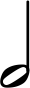
\includegraphics[scale=0.5]{img/half_note}
}
&
\parbox{0.15\linewidth}{
\centering
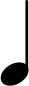
\includegraphics[scale=0.5]{img/quarter_note}
}
&
\parbox{0.15\linewidth}{
\centering
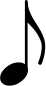
\includegraphics[scale=0.5]{img/eighth_note}
}
&
\parbox{0.15\linewidth}{
\centering
\includegraphics[scale=0.5]{img/meter}
}
\\
A whole note. & A half note. & A quarter note. & An eighth note & A 4/4 time signature\\

\end{tabular}
\end{table}

These durations are grouped together units called bars or measures. The time signature specifies how a bar is subdivided into metrical units. The time signature consists of two numbers written above each other as in table \ref{tab:notation}, when written in text we refer to this as a 4/4 time signature where the first number is the top number and the second number is the bottom number. The top number specifies the number of notes per measure, the bottom number specifies the units of those notes. The time signature is sometimes called meter.

Staff music notation is one of the most widespread representation of rhythmic structure. In the field of rhythm analysis, another structure is popular, called a \textit{metrical grid}, which originally introduced by \citet{lerdahl1983generative} in their Generative Theory of Tonal Music. A metrical grid is a representation that contains several levels, where the lowest level corresponds to the smallest subdivided unit and the highest level corresponds to a bar. A metrical grid representing a 3/4 time signature is shown in figure \ref{fig:grid}. Bars are separated using a horizontal line, $\bullet$ symbols indicate the \textit{downbeats} of each level. The downbeats are the leftmost units metrical unit of a subdivided unit. Level three for example contains one downbeat per bar. Level three is subdivided into three level-two downbeats, the second and third of which is a level-three \textit{upbeat}. Every level-two unit is subdivided into two level-one downbeats, the second of which is a level-two upbeat. 

\begin{figure}[b]
\centering
\hspace{2in}
\begin{tabular}{llllll|llllll|ll}
$\bullet$ &  &  &  &  &  & 		$\bullet$ &  &  &  &  &  & $\bullet$ & Level 3\\ 
$\bullet$ &  & 	$\bullet$ &  & 	$\bullet$ & & 	$\bullet$ & & $\bullet$ &  & $\bullet$ &  & $\bullet$ & Level 2\\
$\bullet$ & 		$\bullet$ & 		$\bullet$ & 		$\bullet$ & $\bullet$ & $\bullet$ & $\bullet$ & $\bullet$ & $\bullet$ & $\bullet$ & $\bullet$ & $\bullet$ & $\bullet$ & Level 1\\
\end{tabular}
\caption{Metrical grid of a 3/4 time signature.}
\label{fig:grid}
\end{figure}

Having now introduced two representations of rhythmic structure, we can turn to some the work done in this field. The most extensive recent study was conducted by \cite{temperley2010modeling}, where he studies the probabilistic properties of rhythmic structures in isolation. It is suggested that rhythm has some probabilistic characteristics that are shared to some extend by a wide range of musical styles. Temperley identifies a number of intuitions about rhythm that seem to be common-practice. These intuitions include the general tendency of onsets to fall on downbeats, the preference for onsets on upbeats to be preceded or followed by a note on the previous or next downbeat and the tendency of long notes to fall on downbeats. 

Temperley proposes six different models intended to be sensitive to these regularities. The adequacy of these models is evaluated by measuring their cross-entropy, using cross-validation on a corpus of European folk songs. Temperley's work shows that it is fairly easy to devise probabilistic models that differentiate common rhythms from less common rhythms. Intuitively, these models explain that not every pattern of onsets that can by described as a valid rhythmic structure will be perceived as a rhythm by humans. 

% Metrical grids?

\section{Performances}
\label{sec:performances}

Rhythmic structure in itself does not imply onsets in absolute time. The common way to relate a rhythmic structure to a performance is by assigning some real duration to a metrical unit. The amount of real time we assign to a metrical duration is usually called the \textit{tempo}. Given a tempo, a rhythmic structure can be converted to a set of \textit{idealised} onset times, also called metronomic onset times. 

When humans perform a rhythm, they deviate from the idealised onset times in several ways. Unless a metronome is used, the tempo will usually fluctuate as the performance progresses. Much of this fluctuation is intentional and is referred to as \textit{musical expression}. Apart from global tempo changes humans deviate from idealised onsets locally as well, even when a metronome is used. 

In general, it is thought that, depending on the competence of the performer, some proportion of this local deviation, is noise but a large proportion of it seems to be systematic. A study by \citet{palmer1989mapping} suggested that global tempo changes are mostly guided by conscious intention. Local deviations in timing and loudness seemed to be partly unconscious. Pianists were for example aware that they articulated certain beats but could not reliably tell whether they did so by playing them louder or by altering their timing. These findings suggest that it is to some extent not even possible to perform rhythm without expression.

It seems thus that whereas global tempo changes may be guided by conscious intentions of phrasing, local expression may be partially unconscious. Another study has shown that there is some regularity in local expression that is linked to rhythmic structure \citep{bengtsson1983analysis}. In Vietnamese waltzes for example, which have almost exclusively a 3/4 or 6/8 meter, it is observed that there is a consistent lengthening of the first upbeat at quarter note level.

Although a performance deviates from the idealised onsets given by the structure and tempo, human listeners are often able to derive the rhythmic structure from a performance and multiple listeners tend to be quite consistent in their interpretations of a performance. In fact, the studies above suggest that deviations from idealised onsets are crucial to perception of structure in rhythm.

%Much of this expression appears to be a highly complicated and irregular process that is influenced by factors as musical style and the `mood' of the music, the audience and the performer. There is a field of research concerned with finding models for musical expression, see for example \citet{widmer2004computational}. Here, we will not concern ourselves with extensive models of expression. Instead, we will suggest that there may be more regular forms of local expression that are the result of a tendency of humans to emphasize downbeats.

Several authors have suggested models that try to mimic this human capacity. \citet{cemgil2000rhythm} propose a system for rhythm quantisation that uses Bayesian modelling to derive the rhythmic structure. Their model tries to optimise the probability of a score given a performance, which can be expressed as the probability of the score (the score model) times the probability of the score given the performance (the rhythm model). The performance model simply penalises performances to the extent that they deviate from metronomic onset times. The model assumes tempo can change and uses a tempo-track (often called tempo-curve) to derive metronomic onset times given local tempo. 

\citet{raphael2002hybrid} proposes another model that is similar to the model in \citet{cemgil2000rhythm}. However, here a graphical probabilistic model is proposed where `score-positions' (relative positions of notes within a measure) are seen as a Markov chain of events where the probability of a score position depends on the probability of a note on that position and the probability of a note on that position preceded by the score-position of the previous note. Another Markov chain of tempo values is generated from the the score positions and finally the exact onset time of each note is dependent on the tempo value, score position of the previous note and score position of the current note.

These models are discussed in \citet{temperley2007music} and it is observed that the actual metrical structure still remains ambiguous in the analyses of these models. Temperley proposes a model of rhythm here that is based on a metrical grid, an unambiguous representation of meter and also contains less parameters than the rather complicated models of \citet{raphael2002hybrid} and \citet{cemgil2000rhythm}. This model is elaborated in \citet{temperley2009unified} where it is integrated into a unified probabilistic model of rhythm, harmony and polyphonic structure.

In this study, a rhythm model is proposed implemented based on what Temperley calls metrical anchoring: the probability of a beat on an upbeat depends on whether a note was played on the preceding or following downbeat, this model is called the hierarchical model by Temperley. Later, in \citet{temperley2010modeling}, this model is compared to other rhythm models and it is shown that it performs adequately. This rhythm model is also based on the notion of a metrical grid and is limited to metrical grids containing four levels and only duple divisions. To deal with the problem of tempo, the model has a parameter that specifies the preferred \textit{tactus level} interval. The tactus level is the level in the metrical grid that corresponds to the beats in a measure (see our discussion of time signatures in section \ref{sec:structure}). The tactus interval is allowed to fluctuate: the probability of a next tactus interval is a normal distribution over the previous one, preferring tactus intervals of the same length.

The notion that rhythmic structure is, as it was suggested before, always performed expressively has been largely ignored by the models described above. In all models, expression was considered additive noise with respect to the idealised onsets given some rhythmic structure and tempo representation. Another criticism of the models above is that they all include one or more parameters that are related to tempo. Estimating local tempo is not trivial: in the case of slightly stretched beats as the result of local expression, the beats following that beat will be considered to deviate from the average tempo of that measure. Defining tempo per beat, seems tedious and hard to do accurately. This may lead us to believe that the concept of tempo in relation to expressively performed rhythms may be misleading. A related view is put forward by \citet{desain1993tempo}, who argue that tempo curves can be misleading concept.

In the next section, we will introduce a model that is completely tempo independent and has the potential to become sensitive to rhythmic structure-dependent local expression.

\section{An Expression-Aware Subdivision-Based Rhythmic Parser}
\label{sec:introducing}

% Therefore we present our expression model the way it is presented

% This approach is based on early work by longuet-higgins.
% We try to use regular expression to our advantage
% Also tempo tracks are weird, given that rhythms are always performed expressively and introduce lots of parameters
% Temperleys unified analysis is cool but also estimates a tactus level that is based on real times and it needs 'pips'
% A performance of Chopin includes huge tempo changes that can be instantaneous. A model needs to be free of any assumptions about tempo.

The approach introduced here is inspired by \citet{longuet1976perception}. In this work, rhythmic structure is represented as subdivision trees rather than staff notation or metrical grids. A subdivision tree represents rhythms as a hierarchical structure where some metrical duration corresponding to the root node is subdivided into child nodes. An example of such a structure is shown in figure \ref{fig:subdivision:a} and three possible staff notation interpretations of the structure in figure \ref{fig:subdivision:b}. Although musicians might play score C slower than score B and score B slower than score A, they are structurally identical and as we have said earlier, our model will be tempo-independent. The different scores are inferred from the tree by defining some level in the tree to be the bar duration.

\begin{figure}[t]
\centering
\subfloat[]{
\label{fig:subdivision:a}
\centering
\Tree
[ .{$\frac{1}{1}$} [ .{$\frac{1}{2}$} [ .{$\frac{1}{4}$} [ .$\bullet$ ] [ .{$\frac{1}{8}$} [ .$\bullet$ ] [ .$\bullet$ ] [ .$\bullet$ ] ] ] [ .{$\frac{1}{4}$} [ .$\bullet$ ] [ .$\bullet$ ] ] ] [ .{$\frac{1}{2}$} [ .{$\frac{1}{4}$} [ .$*$ ] [ .$\bullet$ ] ] [ .$\bullet$ ] ] ] 
}

\subfloat[]{
\label{fig:subdivision:b}
\centering
\begin{tabular}{| l  >{\centering\arraybackslash}m{2in} |}
\hline 
A & 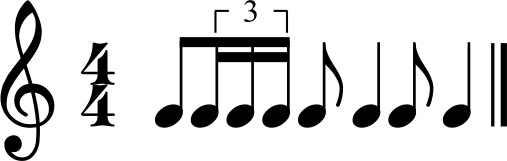
\includegraphics[scale=0.3]{img/subdivision_score1}\\
B & 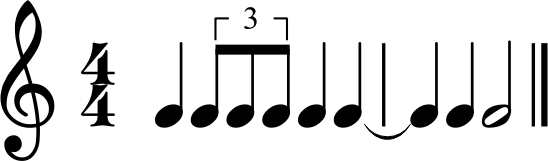
\includegraphics[scale=0.3]{img/subdivision_score2}\\
C & 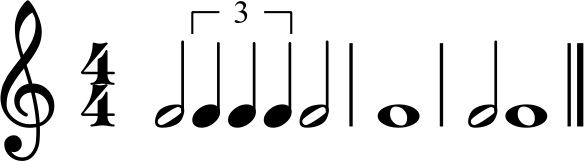
\includegraphics[scale=0.3]{img/subdivision_score3}\\
\hline
\end{tabular}
}
\caption{An analysis and three different score notations of the same musical clich\'e. }
\label{fig:subdivision}
\end{figure}

In staff notation the longest metrical unit is a whole note, which can be lengthened using dotted notation or ties. In the subdivision tree in figure \ref{fig:subdivision}, every node represents some metrical duration which may correspond to notes, bars or multiple bars. Although figure \ref{fig:subdivision} only shows duple and triple subdivisions a metrical unit in the tree can be subdivided into any prime number child-units. We specify two types of leaf-nodes: an onset, which we show as a $\bullet$ symbol in subdivision trees and a tied note, which we show as a $*$ symbol in subdivision trees. Figure \ref{fig:ties} shows how these symbols are interpreted. The $\propto$ symbol means that the expression on the left is proportional to the expression on the right.

\begin{figure}
\centering
\subfloat[A subdivision of a three note rhythm.]{
\parbox{0.25\linewidth}{
\centering
\Tree
[ .{$\frac{1}{1}$} [ .$\bullet$ ] [ .{$\frac{1}{2}$} [ .$\bullet$ ] [ .$\bullet$ ] ] ]
}
$\mathlarger{\mathlarger{\mathlarger{\propto}}}$
\parbox{0.25\linewidth}{
\centering
\includegraphics[scale=0.3]{img/intro1}
}
}

\subfloat[A subdivision tree of a two note rhythm containing a tied note.]{
\parbox{0.25\linewidth}{
\centering
\Tree
[ .{$\frac{1}{1}$} [ .$\bullet$ ] [ .{$\frac{1}{2}$} [ .$*$ ] [ .$\bullet$ ] ] ]
}
$\mathlarger{\mathlarger{\mathlarger{\propto}}}$
\parbox{0.25\linewidth}{
\centering
\includegraphics[scale=0.3]{img/intro2}
}
}
\caption{The interpretation of onsets and ties in subdivision trees.}
\label{fig:ties}
\end{figure}

The approach presented in \citet{longuet1976perception} is a rule-based system that needs to be initialised with a tactus length and some tolerance parameter that specified how much performances where allowed to deviate from metronomic timing. Nowadays, computers are powerful enough to construct probabilistic models based on corpora and to consider a great number of possible structural interpretations of a performance at once. With this in mind, we will briefly introduce our system below before discussing it in detail in the next chapter.

We will boil down a performance to a list of onsets. We think onsets provide enough information to correctly identify rhythmic structure. Therefore, we will from now on talk about onsets rather than notes.

Subdivision trees that describe valid rhythmic structures can be described in a context-free grammar (CFG). An algorithm that determines the hierarchical structure of an input given some CFG is called a parser. We will present a CFG and a parser that constructs hierarchical structures like in figure \ref{fig:subdivision:a} from performances. Our parser will be some variant of a class of efficient parsers called chart-parsers.

Our parser will be guided by a Bayesian model which allows us to describe a probable structure given a performance as the probability of the structure itself, described by a \textit{rhythm model} times the probability that this structure generated the observed performance, described by an \textit{expression model}.

Similar to \cite{temperley2009unified}, we will use a rhythm model that is sensitive to common-practice notions about rhythm. However, instead of his hierarchical model, which is based on metrical grids, we will use a probabilistic context-free grammar (see section \ref{sec:prior}). This model follows naturally from our representation of rhythmic structure.

We have claimed that some structure-related expressive deviations may be regular. Emphasising beats can result in a slight stretching of the duration of the beat. Depending on the style of the music, some beats may be emphasised regularly. In general it seems downbeats are often emphasised. If such stretching does indeed happen regularly, it will result in downbeats at levels near the leaf nodes of the tree to be slightly longer than upbeats. A tempo independent way to look at this is as the ratio of downbeat length and upbeat length. The expression model will assume that the down-/upbeat length ratio can be estimated from a number of features.

To train our rhythm and expression model, we need a corpus of monophonic performances of rhythms annotated with subdivision trees. For this purpose we have constructed a corpus of monophonic jazz melodies, performed by amateur musicians. The corpus was annotated with metrical onset times and subdivision trees were generated using a non-probabilistic version of our parser. This was possible because we could assume the onset times were metronomic.\footnote{Technically, the onsets are specified in metrical units and not metronomic units. However, since our parser is tempo-independent this does not matter.}

Finally, the parser is evaluated on the same corpus. We will use cross-validation to avoid testing on the same data we trained on.
%Representation: subdivision trees
%Context free grammar, parser
%Bayesian model: rhythm model, expression model
%Parameters learned from annotated corpus.
%Expression model: expression ratio
%Advantage of subdivision trees with respect to expression: we always know what the down- and upbeats are.
\chapter{Related Work}
\label{sec:relatedwork}

\begin{itemize}
\item Rhythm quantisation, rhythm models
\end{itemize}


Several authors have suggested that some rhythmic structures are more likely than others. \cite{cemgil2000rhythm} incorporated a notion of rhythmic complexity into their system for music transcription, where the likelihood of a rhythm is inversely proportional to its complexity. Temperley suggests a more thorough description of rhythm likelihood \citep{temperley2010modeling}. In \cite{temperley2009unified} he uses his hierarchical position model in a probabilistic music analysis system. [Explain somewhere why a PCFG captures Temperley's properties of common practice rhythm. If it even does...]. [Honing suggests a few priors somewhere else as well.]

Our hypotheses are represented as subdivision trees. This analysis suggests yet another way of characterising rhythm likelihood, commonly known as a probabilistic context-free grammar(PCFG). 

We will use several priors to evaluate our model. [these priors should be described in detail either here or in the evaluation section]

The likelihood should be a function that measures how well a hypothesis `fits' the observations. The simplest likelihood function is one that assigns zero probability to all hypotheses that do not exactly fit the observations. Such a likelihood would only allow metronomic performances. 

If we want to handle human performances we need to have tolerance for deviations from metronomic timing. In many models [citations], any deviation from metronomic timing is treated as additive noise. Deviations from metronomic timing are penalised using a normal distribution centred around the metronomic onset.

Finding the meter of a piece of music is slightly more complicated than just tracking beats. If we want to know the meter we have to know how many beats are in a bar and which beat is the first beat of a bar. Even if we know all these variables, there can still be an ambiguity between a 6/8 and a 3/4 meter. Furthermore, if we assume that rhythms are performed in perfect time, finding the meter is still nontrivial \cite{temperley2010modeling}. In performances however, rhythms are always performed with some level of expressive timing, that is the length and onset of notes is slightly altered with respect to its notation.

A number of models related to the problem of meter finding have been proposed. Early rule based approaches, like \citet{longuet1976perception}, required manual setting of parameters and were not able to benefit corpora of music. As MIDI allowed music to be represented symbolically and data became more available, models have been presented that can learn from data \citep{cemgil2000rhythm, raphael2002hybrid}. In these models, expression is modelled by allowing the tempo to change and allowing note onsets to be slightly before or metric beats. Although the parameters of these models are learned from data, they do not really contain any model of expression. This may be explained by the fact that they are aimed at classical music, where expression can be highly complex and unpredictable.

Using Bayesian modeling has recently become popular. Temperley proposes a number of models aimed to capture properties of common practice rhythm \citep{temperley2010modeling}. In \citet{temperley2010} these models are objectively compared. Two models, the hierarchical model and the first-order metrical duration model seemed to most effictively capture common-practice rhythm. Below, the hierarchical model will be introduced.

The hierarchical model is a generative model of rhythm production. Temperley's model adopts of the widely used notion of metrical grid \citep{lerdahl1983generative}, where beats are considered to be on different metrical levels. In a four layer metrical grid for example, the length of a bar would be level 3 (whole notes in a 4/4 meter), the first subdivision would be level 2 (half notes in a 4/4 meter), the second level 1 and the third level 0. Temperley's hierarchical model first generates beats on level 3, according to statistics obtained from a corpus, then level two is generated in the same way, level 1 and 0 are generated conditional on their context, that is whether they are preceded or followed by a note on a strong beat (level 3 or 4). Temperley distinguishes four different contexts. Non-anchored notes are not preceded or followed by a note on a strong beat, pre-anchored notes are preceded by a note on a strong beat, post anchored notes are followed by a note on a strong beat and both-anchored notes are preceded and followed by a note on a strong beat. The likelihood of generating level 2 or level 1 notes is now given by the conditional probability of a note on that level given its context.

The hierarchical model is based on intuitions about common-practice rhythm \citep{temperley2010modeling}. Temperley observes for example that notes often fall on strong beats of the metrical grid (the lower levels), notes that fall on strong beats tend to be long and notes on weak beats are often preceded by notes on strong beats. In \citet{temperley2009unified}, a meter-finding application of the hierarchical model is presented. However, this model still does not assume a lot of knowledge about expression and simply penalises notes proportionally to how far their offset is from the metric beat. Again, such a simplification may be justified in the light of highly complex expressive timing in classical music.

The story for Jazz music is quite different. Tempo for example, tends to be quite stable in Jazz performances as it is often played in ensemble and without a conductor. It also seems like it may be possible to make generalisations about the expressive timing in Jazz. Jazz is often played in what is known as \textit{swing} timing. That is, the length of 1/8 notes played unequally and typically described in \textit{swing ratio}. For example, a swing ratio of 2/1 means the 1/8 note on a strong beat (quarter beat) is played with 2/3 of the quarter beat length and the next 1/8 note on a weak beat is played with 1/3 of the quarter beat length.

Exactly how to model a swing ratio is not clear. Empirical studies on professional Jazz percussionists have shown that the swing ratio varies with tempo. \citet{friberg2002swing} suggested that swing ratio scales lenearly with tempo. However, this claim was criticised by \citet{honing2008swing}, who provided evidence that swing ratio does scale with tempo but not linearly. This may be related to claim that expressive timing does not scale linearly with tempo \citep{desain1993tempo, desain1994does}.

Finally, it may be suggested that a simultaneous harmonic analysis may improve the rhythmic analysis. \citet{temperley2009unified} describes how such a combined analysis might be implemented. This may be a fruitful approach but as can be seen in Temperley's work, an independent rhythmic analysis can be easily integrated in such a system. In addition to that, humans typically are able to determine rhythmic structure without hearing the harmony, whereas determining the harmonic structure without the rhythm may be harder. For these reasons, the approach proposed here will focus only on rhythm.
%\section{Motivation}
\label{sec:motivation}


The approach that is proposed works completely independent of tempo. No assumptions are made about the maximum or minimum number of subdivisions. Music transcriptions can be derived from analyses simply by setting a tactus level.

\chapter{Method}
\label{sec:method}

In this chapter, the complete system will be described. A number of definitions are made first in section \ref{sec:definitions}. Section \ref{sec:parser} will introduce a parser that constructs valid rhythmic structures. Section \ref{sec:rejection} will describe the probabilistic elements of the parser. These are elaborated in section \ref{sec:prior} and \ref{sec:likelihood} where respectively the rhythm and expression model are discussed. Section \ref{sec:corpus} will introduce the jazz corpus. Section \ref{sec:training} will describe how the rhythm and expression model are trained on the corpus. Finally, section \ref{sec:implementation} will describe a few details of our implementation of the parser.

\section{Background}
\label{sec:definitions}

We assume that we can represent the performance $P$, of a rhythm as series of note onset times. 
\begin{equation}
\label{eq:performance}
P = [\mathrm{On}_0, \mathrm{On}_1, \cdots, \mathrm{On}_n]
\end{equation}
where $\mathrm{On}_i$ is a note onset. For human listeners, this information is usually enough to correctly identify the rhythmic structure. Other features of the perception, like pitch and note offsets are useful as well, but in many cases, note onsets are sufficient. Note onsets are also the property that rhythms played by any instruments have in common. When a rhythm is performed on a drum for example, pitch and note offsets are practically absent.

We will consider the perceived \textit{rhythm} to be the underlying structure of a performance and the performance a noisy representation of the underlying rhythm. In Western music tradition, a rhythm can be described as a series of subdivision of some metrical unit. The most common subdivisions are duple and triple divisions. Other prime number divisions are allowed as well but are far less common in at least in Western music tradition. When a metrical unit is divided into two or three units, the leftmost unit is, by convention, called the \textit{downbeat}. The other unit(s) are called \textit{upbeat}(s).

A quarter note in a 4/4 time signature for example, is a whole note divided two twice. The first beat of a 4/4 bar is the downbeat at the half note level and every level below. The third beat of the bar is an upbeat at the half note level, since its the second half of a whole note divided by two, but a downbeat at the quarter note level and below. Many authors have used the notion of a metrical grid, introduced by \citet{lerdahl1983generative} in their Generative Theory of Tonal Music, to represent this structure. Another popular representation of rhythmic structure is staff notation. Here we will use a different kind of representation which we will refer to as \textit{subdivision trees}. We will argue that this is a more general representation of rhythm than staff notation or metrical grids. [No timesignatures, irrelevance of tempo curves]

Every node in the subdivision tree represents a metrical duration. Any node can be subdivided into any prime number of subnodes. A node is considered to be non-terminal if it is subdivided and terminal if it is not. There are two types of terminal nodes: an onset, which we will show as $\bullet$ in our graphical representation of trees, and a filler unit, which will be shown as $*$. A filler unit can be either a tied note or a rest. There are no rests in the subdivision trees since we are only looking at onsets. The filler units will be referred to as ties from now on.

The metrical length of a node's child nodes is equal to the length of the node divided by the number of children. We do not need to define the length of the root node, and therefore metrical durations can be expressed relatively as a number of divisions of the root node. We can make a distinction between a \textit{metronomic duration} and a \textit{metrical duration}. Where a metronomic duration is a duration measured in some unit of time and a metrical duration is a duration relative to the root node. 

An example of a well known rhythmic clich\'e and its analysis is shown in figure \ref{fig:subdivision:a} to illustrate the concept of a subdivision tree. The root note is labelled 1/1,  its children are labelled 1/2, etc. These fractions are fractions of the duration of the whole rhythm and are not to be confused with actual whole notes and half notes, which are a consequence of what level of the tree we consider the bar level. The node labels only indicate the division of the total length of the analysis. In order to derive a score from the tree in figure \ref{fig:subdivision:a}, we need to assign some level in the tree to equal a whole bar. Score A in figure \ref{fig:subdivision:b} shows how the first note becomes an eighth note under a 4/4 time signature with the bar duration set to to the root node. Setting the bar duration one level lower results in score B and setting it another level lower results in score C. Hence, a subdivision tree abstracts away time signatures, making it a more general representation than staff notation.

\begin{figure}
\centering
\subfloat[]{
\label{fig:subdivision:a}
\centering
\Tree
[ .{$\frac{1}{1}$} [ .{$\frac{1}{2}$} [ .{$\frac{1}{4}$} [ .$\bullet$ ] [ .{$\frac{1}{8}$} [ .$\bullet$ ] [ .$\bullet$ ] [ .$\bullet$ ] ] ] [ .{$\frac{1}{4}$} [ .$\bullet$ ] [ .$\bullet$ ] ] ] [ .{$\frac{1}{2}$} [ .{$\frac{1}{4}$} [ .$*$ ] [ .$\bullet$ ] ] [ .$\bullet$ ] ] ] 
}

\subfloat[]{
\label{fig:subdivision:b}
\centering
\begin{tabular}{| l  >{\centering\arraybackslash}m{2in} |}
\hline 
A & 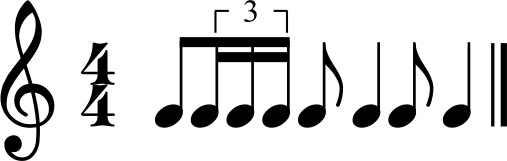
\includegraphics[scale=0.3]{img/subdivision_score1}\\
B & 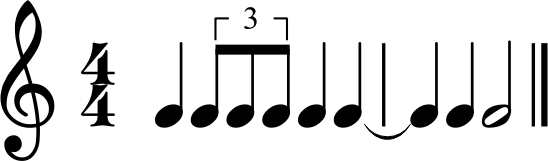
\includegraphics[scale=0.3]{img/subdivision_score2}\\
C & 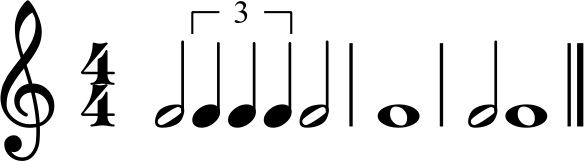
\includegraphics[scale=0.3]{img/subdivision_score3}\\
\hline
\end{tabular}
}
\caption{An analysis and three different score notations of the same musical clich\'e. }
\label{fig:subdivision}
\end{figure}

%When humans perform a rhythm, some information about this underlying structure is encoded in the performance of the rhythm which may be why humans find it usually easy to hear the downbeat. In many music styles, it is common to emphasise the downbeat. It is hypothesised here that this emphasis takes the form of a slight asymmetry in the duration of the downbeat and the duration of the upbeat.

\section{Parsing Rhythms}
\label{sec:parser}

The approach presented here generates the most likely rhythmic structure $R$ underlying a performance $P$, where $R$ is a subdivision tree as described in the previous section and $P$ is a list of onsets as shown in equation \ref{eq:performance}. During this process the parser considers all possible hypotheses of small sub spans of $P$ and retains the most likely ones. This is feasible because we assume that over a few notes, only a small number of hypotheses are worth considering. In this section we will first describe how rhythmic analyses that are structurally sound are generated. After that, we will outline a Bayesian model that defines how we determine whether a hypothesis is likely.

The process of generating hypotheses about performances will be referred to as parsing from now on. Rhythmic analyses will be generated by a slightly modified stochastic CKY chart parser \citep{Younger1967recognition}. The full algorithm and modifications are given in appendix \ref{app:parser}. A small context-free grammar augmented with some constraints will be used to generate subdivision trees. The grammar below constructs subdivision trees $R$ from onsets ($\bullet$) and ties ($*$).
\begin{align}
R &\rightarrow R\: R\\ \notag
R &\rightarrow R\: R\: R\\ \notag
R &\rightarrow \bullet\\ \notag
R &\rightarrow * \notag
\end{align}
We will restrict ourselves to duple and triple subdivisions for this study..

The CKY parser only accepts grammars that are given in the so-called Chomsky normal form (CNF). That is, all rules should be of the form $A \rightarrow B, C$ or $A \rightarrow \alpha$, where $A$, $B$ and $C$ are non-terminal symbols and $\alpha$ is a terminal symbol. Converting the grammar above to CNF results in the following grammar:
\begin{align}
\label{eq:grammar_cnf}
R &\rightarrow R\: R\\ \notag
R &\rightarrow R\: R'\\ \notag
R' &\rightarrow R\: R\\ \notag
R &\rightarrow \bullet\\ \notag
R &\rightarrow * \notag
\end{align}

Two constraints are needed to prevent the parser from generating invalid rhythmical structures. These constraints are: (1) Any set of two or three metrical durations are not allowed to combine if the first one expands directly to an onset and the others do not recursively expand to an onset. (2) Metrical durations are not allowed to combine if none of them recursively contains an onset.

\begin{figure}
\centering
\subfloat[]{
\parbox{0.2\textwidth}{
\Tree
[ .{$\frac{1}{1}$} [ .$\bullet$ ] [ .{$\frac{1}{2}$} [ .$\bullet$ ] [ .$*$ ] ] ]
}
=
\parbox{0.2\textwidth}{
\Tree
[ .{$\frac{1}{1}$} [ .$\bullet$ ] [ .$\bullet$ ] ]
}
}
\qquad
\subfloat[]{
\parbox{0.2\textwidth}{
\Tree
[ .{$\frac{1}{1}$} [ .{$\frac{1}{2}$} [ .$*$ ] [ .$*$ ] ] [ .$\bullet$ ] ] 
}
=
\parbox{0.2\textwidth}{
\Tree
[ .{$\frac{1}{1}$} [ .$*$ ] [ .$\bullet$ ] ] 
}
}
\caption{Redundant tree structures}
\label{fig:constraints}
\end{figure}

The first constraint prevents the parser from generating structures with an onset on the downbeat and a tie on the upbeat. Tying a downbeat to an upbeat would not make sense since a quarter note tied to a quarter note is simply a half note. The second constraint prevents the parser from combining subdivision trees that do not contain onsets. Figure \ref{fig:constraints} illustrates how these structures are redundant.

% Explanation of the chart parser?

This completely defines the parser. At this point however, the parser simply generates all possible interpretations of an onset list of a certain length. The next sections will describe how a probabilistic model is used to reject unlikely interpretations and retain the likely ones.

\section{Hypothesis generation and rejection}
\label{sec:rejection}

Subdivision trees generated by the parser can be seen as hypotheses about the rhythmic structure (some sub-span of) the performance. We will assume that the likelihood of an hypotheses given a set of performed onsets is determined by two factors: One is how well the analysis matches the observed onset times and another is likely the rhythm itself is. [Picture of too detailed versus too simple analyses a la cemgil 2000]. In other words, we want to find the \textit{posterior} probability $P(A|N)$, where $A$ is a rhythm, and $N$ is a list of note onsets. We can formulate this as a generative model where
\begin{equation}
\label{eq:model}
P(R|P) \propto P(P|R)P(R).
\end{equation}

The posterior probability $P(R|P)$ of a rhythm $R$ given a performance $P$ is proportional to the probability that $R$ generated performance $P$, $P(P|R)$, times the probability of $R$ itself, $P(R)$. $P(P|R)$ will be referred to as the \textit{likelihood} of $R$ given $P$ and $P(R)$ will be referred to as the \textit{prior} probability of $R$.

Another way to refer to the prior and the likelihood is as respectively a rhythm model and expression model. The rhythm model should capture intuitions about rhythms, for example that long notes tend to fall on downbeats, that duple divisions are more likely than triple divisions, etcetera. The prior used in this study will be described in section \ref{sec:prior}

The expression model defines how and to what extent we expect onsets deviate from their idealised onsets. In our system, the expression model will be based around one observation, which we shall call the \textit{expression ratio}. The expression ratio is defined as the logarithmic ratio of downbeat length and upbeat length. In metronomic performances, we expect the ratio to be zero for every symbol in the subdivision tree. At low levels, the ratio reflects local expressive timing. A positive value at the quarter note for example indicates that downbeats are played slightly longer than upbeats (for example as a means of emphasising them). At higher levels, above the bar-level, the expression ratio reflects global changes in tempo.

% So no tempo curves are needed

Finally, the chart parser should only keep track of hypotheses that are reasonably sensible. For this purpose, two types of beams are used [REFERENCE?]: First, the per-item likelihood of the hypothesis (see section \ref{sec:training}) should be higher than a certain threshold parameter, called the \textit{beam}. Second, we are now in a position to define what it means for a hypothesis to be sensible: a sensible hypothesis is a hypothesis that has a high posterior probability. After a cell has been filled with hypotheses by the parser (see appendix \ref{app:parser} for more details), the hypotheses are ranked by their posterior probability and only the top-$n$ hypotheses are kept.

Both the rhythm and the expression model will be trained on a corpus of annotated jazz performances that was constructed for this study. The corpus will be described in detail in section \ref{sec:corpus}.

\section{Rhythm model}
\label{sec:prior}

The prior probability of an analysis $R$ should be an indication of how likely $R$ is a priori. Should we only use a hypothesis likelihood to assess the quality of our hypotheses, the parser would produce overly complicated analyses that try to fit the performance as close as possible. This is illustrated in figure \ref{fig:detailed}. By using an rhythm model in parallel with an expression model, the parser is able to balance how well the analysis `fits' the performance and how likely the analysis by itself is.

The subdivision trees that are used in this study suggest a simple rhythm model: a probabilistic context-free grammar (PCFG). A PCFG is a context-free grammar extended with probabilities for every rewrite rule. The probability of a syntax tree, produced by a PCFG can be derived by taking the product of every rule that was applied to construct the tree. In linguistics, PCFGs do not always assign probabilities to rules expanding to terminal symbols (words) since there are too many of them. In our case however, there are only two terminal symbols so we can assign probabilities to rules expanding to onsets or ties as well.

Note that there is only one non-terminal symbol in our grammar, namely $R$, so the probability of a rule expansion is given by
\begin{equation}
P(R \rightarrow S) = P(S) = \frac{\mathrm{count}(S)}{N},
\end{equation}
where S is a string of symbols and N is the total number of $R$ symbols in the training set.


\section{Expression model}
\label{sec:likelihood}
\subsection{Hypothesis representation}
\label{sec:hypothesis_representation}

\begin{figure}
\Tree
[ .{$\frac{1}{1}$} [ .{$\frac{1}{2}$} [ .$\bullet$ ] [ .$\bullet$ ] ] [ .$*$ ] ]
\caption{A rhythmic analysis, which can be represented as the nested list $((\bullet, \bullet), *)$.}
\label{fig:smalltree}
\end{figure}

While a subdivision tree specifies a rhythmic structure, it does not keep track of the onsets associated with the structure. In order to be able to say anything about the likelihood of an analysis, we need to have information about the onsets it contains. Therefore we will introduce a distinction between a rhythmic analysis $R$, produced by the grammar in (\ref{eq:grammar_cnf}) and a \textit{hypothesis} $h$. 

A subdivision tree is essentially a syntax tree, which, as any syntax tree, can be represented as a nested list. The tree in figure \ref{fig:smalltree} for example, can also be written as $((\bullet, \bullet), *)$. Hypotheses have a similar structure but also keep track of onsets on on the down- and upbeats. The 3-tuple below completely specifies a hypothesis.
\begin{align}
h = (H, B, O)\\ \notag
H = [h_0, \cdots, h_d]\\ \notag
B = [b_0, \cdots, b_d]\\ \notag
O = [o_0, \cdots, o_d] \notag
\end{align}
where $d$ is the division of $h$, $H$ is a list of nested hypotheses and $B$ is a list of predicted down- and upbeats that will be constructed using the \textsc{combine} function introduced later in this section. $O$ is a list of actual onsets and may contain $*$ symbols when no onsets are present at some positions. Both $B$ and $O$ only contain onsets on the level of the hypothesis, that is, they contain the down- and upbeat(s) of the hypothesis and their length is always the same as the amount of units the hypothesis divides in. The predicted downbeat of an hypothesis is $B_0$. The predicted upbeats of an hypothesis are $B_i$ where $i > 0$. When a hypothesis governs only a single onset, both $B$ and $O$ may contain $*$ symbols.

A single onset is represented as a hypothesis with zero nested hypotheses: $(\emptyset, [\textrm{On}_i], [\textrm{On}_i])$, where $\textrm{On}_i$ is an absolute onset time at position $i$ in some performance $P$. Similarly, a single tie is represented as: $(\emptyset, [*], [*])$. Combining these hypotheses yields $([(\emptyset, [*], *), (\emptyset, [\textrm{On}_i], \textrm{On}_i)], [*, On_i], [*, On_i])$ (see for example figure \ref{fig:complexonsets:a}). Both the list of predicted beats $B$ and the list of onsets $O$ contain the $*$ symbol here. When this hypothesis combines with other onsets, the \textsc{combine} function will fill in the estimated onsets of $*$ in the list of beats $B$, but not in the list of onsets $O$. When the \textsc{observations} function is introduced in section \ref{sec:observations} it will become clear why the list of onsets $O$ is needed.

Estimating the likelihood of a hypothesis is done in a two-step process. The first step is a bottom-up process where the down- and upbeats of every hypothesis is estimated. This process will be described in section \ref{sec:combination}. The second step is a top down process that generates, given some hypothesis, an observation vector containing feature vector/expression ratio pairs. This process is described in section \ref{sec:observations}. The likelihood of these observations given their feature vectors can be determined after the expression model is trained on a corpus. The training procedure is described in section \ref{sec:training}.

For every observation an expression ratio, a feature vector $\varphi$ will be generated. We have already observed in section \ref{sec:rejection} that the expression ratio reflects different concepts as different levels, therefore one feature we will be using is the \texttt{level} at which the expression ratio was observed. We will use another feature reflecting the \texttt{division} of the metrical unit in which the expression ratio was observed. The resulting feature vector is:
\begin{equation}
\label{eq:features}
\varphi = [\texttt{level}, \texttt{division}].
\end{equation}
\texttt{level} is defined bottom-up, so level one is the deepest level of the tree.


\subsection{Combination}
\label{sec:combination}

A hypothesis is said to \textit{govern} a set of onsets if the hypothesis recursively contains these onsets. The \textsc{combine} function cannot estimate down- and upbeats when of a hypothesis that only governs a single onset. Such hypotheses are treated as a \textit{complex onset}. The hypothesis in figure \ref{fig:complexonsets:a} for example is treated as an onset at relative position $0.5$, the hypothesis in figure \ref{fig:complexonsets:b} is treated as an onset with relative position $0.75$.

\begin{figure}
\centering
\subfloat[complex onset: $0.5$]{
\label{fig:complexonsets:a}
\parbox{4cm}{\centering
\Tree
[ .{$\frac{1}{1}$} [ .$*$ ] [ .$\bullet$ ] ] 
}
}
\subfloat[complex onset: $0.75$]{
\label{fig:complexonsets:b}
\parbox{4cm}{\centering
\Tree
[ .{$\frac{1}{1}$} [ .$*$ ] [ .{$\frac{1}{2}$} [ .$*$ ] [ .$\bullet$ ] ] ] 
}
}
\caption{Complex onsets (single-onset analyses).}
\label{fig:complexonsets}
\end{figure}

The goal of the \textsc{combine} function is to get the best possible estimates of where the up and downbeats of a hypothesis are. The algorithm works roughly as follows. The input is a list $H$ containing two or three hypotheses. These will be the child nodes of the hypothesis that the combine function is building. The algorithm iterates through the list of hypotheses. If a hypothesis is an onset, the position of the onset and the absolute onset are added to \textit{onsets}. The position is a number between 0 and 2 or 0 and 3, depending on the number of hypotheses in $H$. If a hypothesis is a complex onset, its complex position, determined by the function \textsc{complexPostion}, and absolute onset are added to \textit{complexOnsets}. If a hypothesis suggests a downbeat, this downbeat and its position are added to \textit{onsets}.

\begin{algorithm}
\caption{Combine hypotheses}
\label{alg:combination}
\begin{algorithmic}
\Function{combine}{$H$}
	\State $d \leftarrow$ \Call{length}{$H$}
	\State onsets $\leftarrow \emptyset$
	\State complexOnsets $\leftarrow \emptyset$
	\For{$i \leftarrow 0,d$}
		\State $(H', B', O') \leftarrow H_i$
		\If{$H' = \emptyset$ \textbf{and} $B \neq [*]$}
			\State \textbf{append} ($i, H'_i$) \textbf{to} onsets
		\Else
			\If{$B'_0 \neq *$}
				\State \textbf{append} $(i, B'_0)$ \textbf{to} onsets
			\If{$O'_0 \neq *$}
				\State \textbf{append} $(i, O'_0)$ \textbf{to} $O$
			\EndIf
			\Else
				\State $p$, complexOnset $\leftarrow$ \Call{complexPosition}{$H'_i$}
				\State \textbf{append} ($i + p$, complexOnset) \textbf{to} complexOnsets
			\EndIf
		\EndIf
	\EndFor
	\If{\Call{length}{onsets} $\leq 1$}
		\State \textbf{append} complexOnsets \textbf{to} onsets
	\EndIf
	\State $B \leftarrow$ \Call{fill}{onsets, $d$}
	\State \textbf{return} $(H, B, O)$
\EndFunction
\end{algorithmic}
\end{algorithm}

Once the algorithm has iterated thought $H$, the algorithm checks whether there is an onset on the downbeat. If there is not, the \textsc{downbeat} function attempts to estimate the downbeat from the list of onsets. We assume that an interval based on one or more complex positions is less reliable than an interval based on intervals between downbeats. Only if \textit{onsets} contains less than two onsets, \textit{complexOnsets} is added to it. When the combined length of \textit{onsets} and \textit{complexOnsets} is 1, this hypothesis governs only one onset and the list of beats will only contain that onset and one or more ties. If the combined \textit{onsets} and \textit{complexOnsets} contains more than one onset, the \textsc{downbeat} function estimates downbeat from these onsets.

In a practical implementation, every hypothesis should also keep track of the first onset before and after the hypothesis. This can be used later to restrict endlessly adding ties to the hypothesis.

\subsection{Observing the expression ratio}
\label{sec:observations}

The combination process combines hypotheses makes sure that every hypothesis governing more than one note contains an estimated downbeat. This information is used by the \textsc{observations} function to transform a hypothesis $h$ to a list of observed expression ratios with feature vectors. As mentioned before, we define an the expression ratio to be the logarithmic ratio of the observed upbeat and downbeat length.

For any hypothesis $h = (H, B, O)$, we can calculate the expression ratio given that we know the (estimated or actual) onset of the downbeat, $B_0$ and the (estimated or actual) next downbeat. Since a hypothesis can be divided into more than two units, there may be more than one expression ratio per hypothesis. We define the \textit{relative position} of a beat to be zero for the downbeat, one for the first upbeat and two for the second upbeat. The expression ratio for a hypothesis with division $d$, downbeat $d_0$, next downbeat $d_1$, upbeat onset $u$ and its relative position $i$ is calculated in the following fashion:
\begin{align}
\label{eq:expression}
\mbox{expression ratio} &= \log\left(\frac{(O_i - B_0) / i}{(B_1 - O_i) / (d - i)}\right) & \text{for every $i$ where $i > 0$ and $O_i \neq *$.}
\end{align}

The \textsc{observations} function is used to derive downbeat and next downbeat estimates for any hypothesis that contains more than one onset and all the sub-hypotheses it recursively contains. The main intuition of this approach is that downbeat intervals provide the most reliable information about the local tempo. 

The \textsc{observations} function is a top-down recursive function. It is initialised with a hypothesis $h$, the downbeat of $h$ and the next downbeat. Since we have not yet observed the next downbeat for the top-level hypothesis $h$, we simply set it to the division of $h$ times the inter-onset interval of the downbeat and the first upbeat of $h$ (given that $h$ governs more than one onset, the combination process already provided estimates for every beat in $B$). So for a hypothesis $h = (H, B, O)$, the algorithm is initialised as follows: $\textsc{observations}(h, B_0, *, \textsc{length}(H) \times (B_1 - B_0))$.

The \textsc{observations} function is given in algorithm \ref{alg:observations}. The first step of the function is to initialise the estimated length $l$ as the onset of the next downbeat minus the onset of the downbeat. The division $d$ is initialised as the number of nested hypotheses (which is equivalent to the length of $H$, $B$ or $O$). Then, the set of feature vector/expression ratio pairs $S$ is initialised as an empty set. Finally the $*$ symbol is appended to the list of onsets.

Now the algorithm iterates through all every beat in the hypothesis (in this study there are can be no more than three beats in a hypothesis). For every beat position $i$ where $i > 0$ and $O_i \neq *$ the expression ratio is calculated as in equation \ref{eq:expression}. The requirements $i > 0$ and $O_i \neq *$ ensure that the expression ratio is only calculated for upbeats that contain actual onsets. 

For every beat position in $h$, the algorithm will calculate the downbeat and next downbeat for the nested hypothesis at that position, these values are stored in $b_{\mathrm{down}}$ and $b_{\mathrm{up}}$. 
For some beat position $i$, where $0 < i < d$, $b_{\mathrm{down}}$ is estimated by
\begin{equation}
\label{eq:beatonset}
b_{\mathrm{down}} = \mathrm{downbeat} + l * i/d.
\end{equation}
If an onset has been estimated by the combination process, which indicated by $B_i \neq *$, this onset is used instead. Since the combination process will always have estimated onsets for $h$s governing more than one onset, equation \ref{eq:beatonset} is only used when $h$ governs a single onset.

Given $b_{\mathrm{down}}$ the position of the next downbeat, $b_{\mathrm{up}}$ is estimated by:
\begin{equation}
b_{\mathrm{up}} = b_{\mathrm{down}} + l/d.
\end{equation}
This estimate should be equivalent to the onset at position $i+1$. If there is an onset at position $i+1$, this onset is preferred to the actual onset.

Finally, the recursive step of the algorithm calls \textsc{observations}($h', b_{\mathrm{down}}, b_{\mathrm{up}}$) for every nested hypothesis $h'$ of $h$. The algorithm stops and returns an empty set when $h$ contains no nested hypothesis, which means it represents an onset or tie.


\begin{algorithm}
\caption{Generate observations}
\label{alg:observations}
\begin{algorithmic}
\Function{observations}{$h$, downbeat, nextDownbeat}
	\State $H, B, O \leftarrow h$
	\State $d \leftarrow$ \Call{length}{$H$}
	\State $l \leftarrow$ nextDownbeat - downbeat
	\State $S \leftarrow \emptyset$
	\State \textbf{append} * \textbf{to} $O$
	\For {$i \leftarrow 0,d$}
		\If {$O_i \neq *$ \textbf{and} $i \neq 0$}
			\State $\varphi \leftarrow$ (\Call{depth}{$h$}, $d$)
			\State $r \leftarrow$ \Call{expression\textunderscore ratio}{downbeat, nextDownbeat, $B_i$, $i$, $d$}
			\State \textbf{append} ($\varphi$, r) \textbf{to} $S$
		\EndIf	
		\State $H', B', O' \leftarrow H_i$
		\If {$H' \neq \emptyset$}
			\State $b_{\mathrm{down}} \leftarrow \mathrm{downbeat} + l * i/d$
			\If {$B_i \neq *$}
				\State $b_{\mathrm{down}} \leftarrow B_i$
			\EndIf
			\State $b_{\mathrm{up}} \leftarrow b_{\mathrm{down}} + l/d$
			\If {$O_{i+1} \neq *$}
				\State $b_{\mathrm{up}} \leftarrow O_{i+1}$
			\EndIf
			\State \textbf{append} \Call{observations}{$(H', B', O'), b_{\mathrm{down}}, b_{\mathrm{up}}$} \textbf{to} $S$
		\EndIf
	\EndFor
	\State \textbf{return} $S$
\EndFunction
\end{algorithmic}
\end{algorithm}



%Constraints of the corpusparser (a parser that only allows metronomic performances)

%Single note analysis constraints

%Constraint in adding ties


%Introducing triple divisions introduces ambiguities between triple divisions or more complicated constructions of duple divisions (that are quite unlikely).

\section{Data Preparation}
\label{sec:corpus}

To train the parser's rhythm model and expression model, a corpus of amateur jazz performances was prepared. The corpus contains jazz and latin standards that were scraped off the the web by \citet{Wild:10}. The performances are generally of good quality and are played in a relatively constant tempo. In its original form, the corpus was a set of multi-track MIDI files containing both tracks played by a human performer and tracks generated by a computer in metronomic time.

MIDI files represent music as a list of note-on and note-off events, corresponding to key presses and key releases. Every event has the parameters pitch, velocity and delta-time. Delta-time specifies the time between this events and the last one, pitch is the pitch of the key that was pressed, velocity is the velocity with which the key was pressed or released.

%Our parser will be trained and evaluated on monophonic jazz melodies, played by a human performer. Monophonic tracks that were likely to be played by humans were filtered out automatically. This was done by assuming that tracks played by humans contained a lot of variation in onset velocity and in inter-onset intervals due to imperfect timing. From this subset of performed tracks, tracks containing melodies where selected by hand.

After the filtering process, 20 tracks were left containing unique performances of 12 different melodies. These MIDI files where converted to note lists of the following format:
\begin{align*}
N &= [n_0, n_1, \cdots, n_N],\\
n_i &= (\mathrm{On}_i, \mathrm{Pitch}_i, \mathrm{Velocity}_i),
\end{align*}
where $N$ is a note list containing notes $n_0$ to $n_N$, $\mathrm{On}_i$, $\mathrm{Pitch}_i$ and $\mathrm{Velocity}_i$ is the onset time in micro seconds, pitch and velocity of the $i^{\mathrm{th}}$ note. A very simple annotation format was chosen: a list of metrical onsets, measured in quarter notes, with pointers to the corresponding notes in $N$. There are three types of annotations: an onset, a grace note and a rest. Although this study will ignore grace notes and rests, they are included for completeness and potential future use of the corpus.

An annotation $A$, corresponding to note list $N$ has the following format:
\begin{align*}
A &= [a_0, a_1, \cdots, a_N],\\
a_j &= (\mathrm{Position}_j, \mathrm{Pointer}_j, \mathrm{Type}_j),
\end{align*}
where $\mathrm{Position}_j$ is a metrical position, measured in quarter notes, $\mathrm{Pointer}_j$ is a pointer that points to the index of the corresponding note in the note list and $\mathrm{Type}_j$ indicates whether this annotation is an onset, a grace note or a rest. Since rests are not included in the note list, their pointer is irrelevant and points to zero. 

Some extra information is added to the annotation when it is stored. The annotation $A$ is stored in a 3-tuple $(T, t, A)$, where $t$ is the tempo in beats per minute and $T$ is the time signature. The time signature contains the number of beats per measure, or measure division $d$ and the number by which we have to divide 1 to get the units of those beats $u$, where $u$ can be any positive real number (although $u$ is almost always a power of 2). 
\begin{equation*}
T = (d, u)
\end{equation*}
This representation is identical to the musical representation of time signature. The information in the time signature combined with onsets measured in quarter notes can be used to derive the measure number of every onset in the annotation. To do so, quarter notes ($q$) are first converted to beats ($b$) as follows: $b = qu/4$. A position measured in beats can then be converted to a position measured in bars ($m$) like so: $m = b/d$

Many performances in the corpus where played in swing. Although swing may refer to many intentional deviations from metronomic timing, a very common one is to play notes that are notated as eighth notes as eighth note triplets, the so-called `shuffle'. This is illustrated in figure \ref{fig:swing}. The score usually notates swung notes as in figure \ref{fig:swing:a}, whereas the notes are played as in figure \ref{fig:swing:b} and \ref{fig:swing:c}. Writing swung notes as in \ref{fig:swing:a} is just a notational convention, and often the scores contain instructions to play eighth notes as in figure \ref{fig:swing:b}.

The manual annotation process resulted in lists of metrical onset times. Combined with the time signature and tempo information, the metrical onset times can be converted to any metrical unit and to metronomic onset times. Deriving te subdivision trees from this information was done semi-automatically. A simple parser with a flat prior and a likelihood function that only allowed metronomic timing was used to generate parses for every item in the corpus. From these results correct parses where selected by hand. A subdivision tree for the swing example is shown in figure \ref{fig:swing:c}. 


\begin{figure}
\centering
\subfloat[Rhythm notation]{
\label{fig:swing:a}
\centering
\begin{tabular}{|c|}
\hline
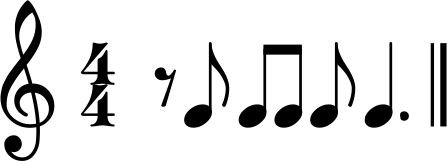
\includegraphics[scale=0.3]{img/aint_misbehavin}\\
\hline
\end{tabular}
}
\\
\subfloat[Annotation]{
\label{fig:swing:b}
\centering
\begin{tabular}{|c|}
\hline
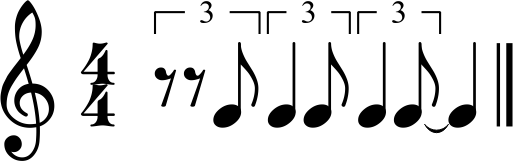
\includegraphics[scale=0.3]{img/aint_misbehavin_swung}\\
\hline
\end{tabular}
}
\\
\subfloat[Parsetree]{
\label{fig:swing:c}
\centering
\Tree 
[ .{$\frac{1}{1}$} [ .{$\frac{1}{2}$} [ .{$\frac{1}{4}$} [ .$*$ ] [ .$*$ ] [ .$\bullet$ ] ] [ .{$\frac{1}{4}$} [ .$\bullet$ ] [ .$*$ ] [ .$\bullet$ ] ] ] [ .{$\frac{1}{2}$} [ .{$\frac{1}{4}$} [ .$\bullet$ ] [ .$*$ ] [ .$\bullet$ ] ] [ .$*$ ] ] ]
}
\caption{Swung notes.}
\end{figure}

The result of this process for Thelonious Monk's standard Blue Monk is shown in table \ref{tab:annotation}.

\begin{table}
\caption{A performance of the first two bars of Thelonious Monk's Blue Monk, the corresponding metrical onsets, rhythmic analysis and score generated from the analysis.}
\label{tab:annotation}
\begin{tabular}{|l|}
\hline

\parbox{\linewidth}{
The performance onsets in milliseconds.
}\\

$P = [32, 348, 504, 836, 1940, 2240, 2420, 2728]$\\

\hline

\parbox{\linewidth}{
Metrical onsets in quarter notes. Triple divisions are rounded to two digits.
}\\

$ A = [0.0, 0.66, 1.0, 1.66, 4.0, 4.66, 5.0, 5.66]$\\

\hline

\parbox{\linewidth}{
Rhythmic analysis generated by a simple parser and selected by hand.
}\\

\Tree
[ .{$\frac{1}{1}$} [ .{$\frac{1}{2}$} [ .{$\frac{1}{4}$} [ .{$\frac{1}{8}$} [ .$\bullet$ ] [ .$*$ ] [ .$\bullet$ ] ] [ .{$\frac{1}{8}$} [ .$\bullet$ ] [ .$*$ ] [ .$\bullet$ ] ] ] [ .$*$ ] ] [ .{$\frac{1}{2}$} [ .{$\frac{1}{4}$} [ .{$\frac{1}{8}$} [ .$\bullet$ ] [ .$*$ ] [ .$\bullet$ ] ] [ .{$\frac{1}{8}$} [ .$\bullet$ ] [ .$*$ ] [ .$\bullet$ ] ] ] [ .$*$ ] ] ]
\\

\hline

\parbox{\linewidth}{
Score generated from the subdivision tree combined with pitch information. The bar duration was set to level 1/2 of the subdivision tree.}\\

\includegraphics[scale=0.4]{img/blue_monk}\\

\hline
\end{tabular}
\end{table}


\section{Training}
\label{sec:training}

The model is trained using maximum likelihood estimation. First, for all items in the train set, the observed parameters are and their corresponding feature vectors, the resulting feature vector/parameter pairs $(\phi, p)$ are stored in a set S. Second, we train two parameter vectors, $\mu$ and $\sigma$ to contain the expected expression ratio $r$ and standard deviation of $r$ for every feature vector $\phi$ like so:
\begin{align}
\label{eq:training}
\mu_\phi &= \frac{1}{|S|} \sum_{(p | (p, \phi) \in S))} p, \\ 
\sigma_\phi &= \frac{1}{|S|} \sum_{(p | (p, \phi) \in S)} (\mu - p)^2. \notag
\end{align}
Since we use a very simple feature vector, these parameters do not need to be smoothed.

Given the parameter vectors $\mu$ and $\sigma$, estimated by \ref{eq:training}, the likelihood of a set of observations $S$ containing feature/expression ratio pairs $(\varphi, r)$, observed in some hypothesis $h$ is given by:
\begin{equation}
\label{eq:h_likelihood}
\mathcal{L}(S|\mu, \sigma) \propto \prod_{(\varphi, r) \in S} \exp\left(-\frac{(\mu_\varphi - r)^2}{2\sigma_\varphi^2}\right).
\end{equation}

As mentioned in section \ref{sec:rejection}, a hypothesis is rejected if the per-item likelihood is lower than a certain threshold, the beam parameter. The per-item likelihood is defined as

\begin{equation}
\label{eq:per_obs_likelihood}
\mathcal{L}(S| \mu, \sigma) \mbox{ per item } \propto \exp\left(-\frac{1}{|S|}\sum_{(\varphi, r) \in S} \frac{(\mu_\varphi - r)^2}{2\sigma_\varphi^2}\right).
\end{equation}

The beam parameter is set by taking the minimum value of the per-item likelihood of each subdivision tree in the train set. 

\section{Implementation}
\label{sec:implementation}

To make the parser computationally tractable, a few optimisations were needed. It was already mentioned that the parser uses a beam parameter to reject unlikely hypotheses. In addition to that a few extra measures had to be taken.

First of all, the \textsc{observations} function returns no parameters for hypotheses containing a single onset (complex onsets). Their probability is always one and theoretically ties could be added endlessly. To restrict this the parser maintains a small list of allowed single note analyses. This list is compiled by taking all single-note analyses found in the labelled corpus.

Second of all, the corpus contains only 4/4 time signatures, therefore triple divisions are allowed only at note level. All allowed triple divisions are shown in figure \ref{fig:triples}. 

\begin{figure}
$\bullet$
\Tree
[ .{$\frac{1}{1}$} [ .$*$ ] [ .$\bullet$ ] ] 
\Tree
[ .{$\frac{1}{1}$} [ .$*$ ] [ .$*$ ] [ .$\bullet$ ] ] 
\Tree
[ .{$\frac{1}{1}$} [ .$*$ ] [ .{$\frac{1}{2}$} [ .$*$ ] [ .$\bullet$ ] ] ] 
\Tree
[ .{$\frac{1}{1}$} [ .$*$ ] [ .{$\frac{1}{2}$} [ .{$\frac{1}{4}$} [ .$*$ ] [ .$\bullet$ ] ] [ .$*$ ] ] ] 
\caption{Some of the allowed single-note analyses.}
\label{fig:singlenotes}
\end{figure}

\begin{figure}
\Tree
[ .{$\frac{1}{1}$} [ .$*$ ] [ .$*$ ] [ .$\bullet$ ] ] 
\Tree
[ .{$\frac{1}{1}$} [ .$\bullet$ ] [ .$*$ ] [ .$\bullet$ ] ]
\Tree 
[ .{$\frac{1}{1}$} [ .$\bullet$ ] [ .$\bullet$ ] [ .$\bullet$ ] ]
\caption{Allowed triple divisions.}
\label{fig:triples}
\end{figure}
% Beam
% Triple divisions
% Best-n
% Max depth
%
% Chart parsing, beam, prior, likelihood, 

\chapter{Evaluation}
\label{sec:evaluation}

%N-fold cross-validation with flat prior, complexity, depth, pcfg or temperley's prior
%Use different likelihoods: Additive noise, downbeat stretching, louder downbeats

This chapter will first give an overview of how we will evaluate the parser. The rest of this chapter is structured as follows: An overview of the evaluation criteria is given in section \ref{sec:criteria} and the evaluation measure will be explained in section \ref{sec:measure}. 

The parser produces a ranked list of hypotheses. The rhythmic analysis $R$ that corresponds to the most highly ranked hypothesis is assumed to be the parser's interpretation of its input. A parser output $R$ will be evaluated against a gold-standard parse $R^*$ from the corpus by an evaluation measure function. 

We cannot afford to keep a completely separate test set since our corpus is fairly small. Therefore we will train the models on different training sets and evaluate them on small parts of the corpus left out of the training set. This process is known as cross-validation. For $n$-fold cross-validation, the corpus is divided into $n$ equal parts, a training set is constructed from $n-1$ of these parts and a test set is constructed of one of these parts. This is done $n$ times and the parts sampled randomly from the corpus. When dividing into $n$ random sampled parts, performances are treated as whole units. Since there are twenty different performances in the corpus, using 10-fold cross validation results in training sets of eighteen performances that will be evaluated on test sets of two performances.

Furthermore, some performances contain over a hundred onsets. The parser is too slow to parse performances longer than around thirty onsets. Therefore the parser will be tested on small slices of performances, consisting of the first few notes of a performance with some preferred length.

Our subdivision trees can only represent performances with a length, measured in whatever metrical unit, that is a power of two. If a performance is for example three bars long, the subdivision tree will represent a fourth bar as a tie. To make evaluation simpler, the test performances are restricted to have lengths that are a power of two. This is done by selecting, given some preferred length, the leftmost nested subdivision tree that contains a number of onsets closest to the preferred length. To do this, we use the subdivision trees in our corpus.

\section{Criteria}
\label{sec:criteria}

To assess the quality of a parser output we will look at how many properties of the gold-standard rhythm were analysed correctly and how many properties of the parse occur in the gold standard rhythm. The subdivision trees describe two properties of rhythm: the location of the down- and upbeats, which is also called the \textit{phase}, and the subdivision pattern, which provides information about the time signature. The evaluation measure should somehow measure the extend to which the parser output is consistent with the gold standard in terms of subdivision and down- and upbeat locations. 

A parser output may be consistent with some aspects of the gold-standard but inconsistent with others. In figure \ref{fig:div_error} for example, the parser correctly identified the downbeat but incorrectly assumed a triple division. It is also possible that the parser correctly identifies the divisions but incorrectly identifies the phase, examples of these kind of errors are shown in figure \ref{fig:phase_error}. Note that a phase error at the deepest level is more severe than a phase error at a higher level. If the phase is incorrect at the deepest level, every downbeat will be identified as an upbeat and vice-versa. If the phase is incorrect at a higher level, the down- and upbeats at the lowest level are still correct. This can be understood intuitively as well: a phase error at the lowest level is more severe since it makes the entire rhythm syncopated, for a phase error at a higher level, the notes on the lower levels would still be in phase.

Notably, figure \ref{fig:phase_error} introduces rests in the parse trees. Rests are necessary to represent that the last note is a quarter note and not a whole note. The parser introduced in in this thesis \ref{sec:method} does not handle rests. This issue is discussed further in chapter \ref{sec:rests}.
\begin{figure}
\centering
\subfloat[Gold-standard.]{
\parbox[3cm]{0.5\linewidth}{
\Tree
[ .{$\frac{1}{1}$} [ .$\bullet$ ] [ .$\bullet$ ] ]
}
}
\subfloat[Parser output.]{
\parbox[3cm]{0.5\linewidth}{
\Tree
[ .{$\frac{1}{1}$} [ .$\bullet$ ] [ .$*$ ] [ .$\bullet$ ] ] 
}
}
\caption{An example of incorrect division detection.}
\label{fig:div_error}
\end{figure}


\begin{figure}
\subfloat[Gold-standard.]{
\label{fig:precision_error:a}
\parbox{0.33\linewidth}{
\Tree
[ .{$\frac{1}{1}$} [ .{$\frac{1}{2}$} [ .$\bullet$ ] [ .$\bullet$ ] ] [ .{$\frac{1}{2}$} [ .$\bullet$ ] [ .$\bullet$ ] ] ]
}
}
\centering
\subfloat[]{
\parbox{0.33\linewidth}{
\label{fig:precision_error:b}
\Tree
[ .{$\frac{1}{1}$} [ .{$\frac{1}{2}$} [ .$\bullet$ ] [ .$\bullet$ ] ] [ .{$\frac{1}{2}$} [ .{$\frac{1}{4}$} [ .$*$ ] [ .$\bullet$ ] ] [ .$\bullet$ ] ] ]
}
}
\subfloat[]{
\label{fig:precision_error:c}
\parbox{0.33\linewidth}{
\Tree
[ .{$\frac{1}{1}$} [ .{$\frac{1}{2}$} [ .$\bullet$ ] [ .{$\frac{1}{4}$} [ .{$\frac{1}{8}$} [ .$*$ ] [ .$\bullet$ ] ] [ .$*$ ] ] ] [ .{$\frac{1}{2}$} [ .$\bullet$ ] [ .$\bullet$ ] ] ]
}
}
\caption{An example of too detailed analyses (resulting in a lower precision)}
\label{fig:precision_error}
\end{figure}

\begin{figure}
\subfloat[]{
\parbox{0.33\linewidth}{
\Tree
[ .{$\frac{1}{1}$} [ .{$\frac{1}{2}$} [ .$\bullet$ ] [ .$\bullet$ ] ] [ .{$\frac{1}{2}$} [ .$\bullet$ ] [ .$\bullet$ ] ] ]
}
}
\subfloat[Gold-standard.]{
\parbox{0.33\linewidth}{
\Tree
[ .{$\frac{1}{1}$} [ .{$\frac{1}{2}$} [ .$\bullet$ ] [ .$\bullet$ ] ] [ .{$\frac{1}{2}$} [ .{$\frac{1}{4}$} [ .$*$ ] [ .$\bullet$ ] ] [ .$\bullet$ ] ] ]
}
}
\centering
\caption{An example of too simple analyses (resulting in a lower recall).}
\label{fig:recall_error}
\end{figure}



\begin{figure}[t]
\subfloat[Gold-standard.]{
\label{fig:phase_error:a}
\parbox{0.2\linewidth}{
\Tree
[ .{$\frac{1}{1}$} [ .{$\frac{1}{2}$} [ .$\bullet$ ] [ .$\bullet$ ] ] [ .{$\frac{1}{2}$} [ .$\bullet$ ] [ .$\bullet$ ] ] ]
}
}
\centering
\subfloat[Phase error at the half note level]{
\label{fig:phase_error:b}
\parbox{0.3\linewidth}{
\Tree
[ .{$\frac{1}{1}$} [ .{$\frac{1}{2}$} [ .$*$ ] [ .{$\frac{1}{4}$} [ .$\bullet$ ] [ .$\bullet$ ] ] ] [ .{$\frac{1}{2}$} [ .{$\frac{1}{4}$} [ .$\bullet$ ] [ .$\bullet$ ] ] [ .$*$ ] ] ]
}
}
\subfloat[Lowest level phase error (most severe).]{
\label{fig:phase_error:c}
\parbox{0.5\linewidth}{
\Tree
[ .{$\frac{1}{1}$} [ .{$\frac{1}{2}$} [ .{$\frac{1}{4}$} [ .$*$ ] [ .$\bullet$ ] ] [ .{$\frac{1}{4}$} [ .$\bullet$ ] [ .$\bullet$ ] ] ] [ .{$\frac{1}{2}$} [ .{$\frac{1}{4}$} [ .$\bullet$ ] [ .Rest ] ] [ .Rest ] ] ]
}
}
\caption{An example incorrect phase detection. See section \ref{sec:discussion} for why there are rests in this subdivision tree.}
\label{fig:phase_error}
\end{figure}

\section{Evaluation Measure}
\label{sec:measure}

The precision and recall of the parser are measured as follows: The precision is the number of subdivisions and down- and upbeats in the parser output that were correctly identified with respect to the gold-standard, divided by the total number of subdivisions and down- and upbeats in the parser output. The recall is the number of subdivisions and down- and upbeats in the gold-standard that are correctly identified by the parser output, divided by the total amount of subdivisions and down- and upbeats in the gold-standard.

To measure these quantities, every onset governed by $R$ and $R^*$ is converted to a list of claims that this onset makes about the structure. For example, the first quarter note of a 4/4 measure claims to be a downbeat at the half note level and a downbeat at the quarter note level (see for example figure \ref{fig:phase_error:a}). The second quarter note claims to be governed by a downbeat at the half note level and to be an upbeat at the quarter note level. The third onset claims to be an upbeat at the half note level and a downbeat at the quarter note level. 

An evaluation that uses these kinds of lists penalises phase errors at the lower levels more severe than phase errors at higher levels. Given the gold-standard in figure \ref{fig:phase_error:a}, consider the following hypothetical errors in the parser output: Should the phase be wrong at the quarter note level (figure \ref{fig:phase_error:b}), a downbeat at the quarter note level becomes  an upbeat, however, the downbeat would still be governed by the downbeat at the half note level. Should the phase be wrong at the half note level (figure, \ref{fig:phase_error:c}), the down- and upbeats at the quarter note level are still correct.

There are two issues with the evaluation as suggested above. First, since every onset lists all claims it implies at higher levels, the parser will get points for divisions at higher levels multiple times. Second, figure \ref{fig:phase_error} shows that a phase error can lead to another level to be added to the tree, which introduces an inconsistency in the interpretation of levels between the parse tree and the gold-standard. 

The first issue is remedied by keeping a list of parser decisions that have been accounted for. If the first onset in figure \ref{fig:phase_error:a} claims a downbeat at the half note level and a downbeat at the quarter note level, both of these claims are added to a list of claimed facts. The second onset claims an upbeat at the quarter note level and a downbeat at the half note level. Since the downbeat at the half note level is already the list of claimed facts it will not be counted again.

To reiterate the first paragraph of this section more concretely, we define the evaluation function \textsc{score}($R, R'$) which counts the number of claims that are shared by $R$ and $R'$ and divides that by the total number of claims in $R$. The precision is defined as the number of claims in $R$ that appear in the claims of $R^*$ as well, divided by the total number of claims in $R$, so:
\begin{equation}
\label{eq:precision}
\mathrm{precision} = \textsc{score}(R, R^*).
\end{equation}
Similarly, the recall is defined as:
\begin{equation}
\label{eq:recall}
\mathrm{recall} = \textsc{score}(R^*, R).
\end{equation}

Consider the example in figure \ref{fig:precision_error}. The current evaluation assigns a precision of $\frac{6}{7}$ and a recall of $\frac{6}{6}$ to the parse in figure \ref{fig:precision_error:a}. This implies that a total of $6$ claims are made by the gold-standard. These are: the four down- and upbeats at the quarter note level and one downbeat and one upbeat at the half note level. The parse in figure \ref{fig:precision_error:b} makes the same claims but also claims an upbeat at the eighth note level, which is incorrect.

We have not addressed the second issue yet. That is, we are not sure if the top level of $R$ corresponds to the top level of $R^*$. Either of those levels may have been added as a result of a different phase in $R$ and $R^*$. The only solution seems to be to consider three scenarios, illustrated by figure \ref{fig:phase_levels}: (1) No extra levels have been added and the levels in $R$ are consistent with the levels in $R^*$. (2) Let $R^*$ be figure \ref{fig:phase_levels:a} and $R$ be figure \ref{fig:phase_levels:c}, then a phase error resulted in an extra level in $R$. (3) Let $R^*$ be figure \ref{fig:phase_levels:c} and $R$ be figure \ref{fig:phase_error:a}, then a phase error resulted in one level less in $R$. 


\begin{figure}
\subfloat[]{
\label{fig:phase_levels:a}
\parbox{0.3\linewidth}{
\Tree
[ .{$\frac{1}{1}$} [ .$\bullet$ ] [ .$\bullet$ ] ] 
}
}
\subfloat[]{
\label{fig:phase_levels:b}
\parbox{0.3\linewidth}{
\Tree
[ .{$\frac{1}{1}$} [ .{$\frac{1}{2}$} [ .$\bullet$ ] [ .$\bullet$ ] ] [ .$*$ ] ]
}
}
\subfloat[]{
\label{fig:phase_levels:c}
\parbox{0.3\linewidth}{
\Tree
[ .{$\frac{1}{1}$} [ .{$\frac{1}{2}$} [ .$*$ ] [ .$\bullet$ ] ] [ .{$\frac{1}{2}$} [ .$\bullet$ ] [ .$*$ ] ] ]
}
}
\caption{Extra levels added by phase errors}
\label{fig:phase_levels}
\end{figure}

If we want to get a valid precision and recall in scenario (2), we should convert $R$ to the tree in figure \ref{fig:phase_levels:b} by adding a top-level tie. In scenario (3) we want to convert $R^*$ to the tree in figure \ref{fig:phase_levels:b} by adding a top-level tie. This suggests three scenarios for evaluation: (1) evaluate $R$ against $R^*$, (2) evaluate $(R, *)$ against $R^*$ and (3) evaluate $R$ against $(R^*, *)$. 

The evaluation function in its final form is:
\begin{align}
\label{eq:evaluation}
&\mathrm{precision} = \textsc{max}(\textsc{score}(R, R^*), \textsc{score}((R, *), R^*), \textsc{score}(R, (R^*, *))),\\
&\mathrm{recall} = \textsc{max}(\textsc{score}(R^*, R), \textsc{score}((R^*, *), R), \textsc{score}(R^*, (R, *))).
\end{align}


% Training and testsets

% Corpus and training and test set sizes (first 4 bars)



%\chapter{Experiments and Results}
\label{sec:results}

% Evaluation of the pcfg prior:
% Show the pcfg model and how it prefers long notes on downbeats and how it penalises syncopation.
First, we will train the rhythm and expression model on the entire jazz corpus as we described in section \ref{sec:training} and analyse the results. Second, we will use 10-fold cross validation to evaluate the performance of the parser on the corpus. We will compare the expression model presented here to an expression model that treats expression as additive noise. That is, for any feature vector $\mu_\varphi$ is set to zero and $\sigma_\varphi$ is set to a small value.

\section{Rhythm and Expression Model}

The rhythm and expression model, trained on the entire jazz corpus are shown in table \ref{tab:models}. 

\begin{table}
\caption{The rhythm and expression model, trained on the entire jazz corpus.}
\label{tab:models}
\centering
\subfloat[The rhythm model.]{
\label{tab:rhythm}
\begin{tabular}{ll}
\hline
\textbf{Rule}& \textbf{Probability}\\
\hline
\hline
$R \rightarrow \bullet\; \bullet$ & 0.061\\
$R \rightarrow *\; \bullet$ & 0.027\\
$R \rightarrow R\; R$ & 0.392\\
$R \rightarrow \bullet\; R$ & 0.057\\
$R \rightarrow R\; \bullet$ & 0.022\\
$R \rightarrow *\; R$ & 0.069\\
$R \rightarrow R\; *$ & 0.061\\
$R \rightarrow \bullet\; \bullet\; \bullet$ & 0.013\\
$R \rightarrow \bullet\; *\; \bullet$ & 0.164\\
$R \rightarrow *\; *\; \bullet$ & 0.134\\
\hline
\end{tabular}
}
\subfloat[The expression model.]{
\label{tab:expression}
\begin{tabular}{lll}
\hline
$\varphi = [\texttt{level}, \texttt{division}]$ & $\mu_\varphi$ & $\sigma_\varphi$\\
\hline
\hline
$[1, 2]$ & $7.926 x 10^{-2}$ & $3.391 x 10^{-2}$\\
$[1, 3]$ & $-6.323 x 10^{-2}$ & $0.656$\\
$[2, 2]$ & $-4.68 x 10^{-3}$ & $2.184 x 10^{-2}$\\
$[3, 2]$ & $5.565 x 10^{-3}$ & $9.422 x 10^{-3}$\\
$[4, 2]$ & $4.797 x 10^{-3}$ & $9.824 x 10^{-3}$\\
$[5, 2]$ & $-3.391 x 10^{-3}$ & $1.887 x 10^{-2}$\\
$[6, 2]$ & $-7.539 x 10^{-5}$ & $1.375 x 10^{-3}$\\
$[7, 2]$ & $-8.029 x 10^{-3}$ & $1.223 x 10^{-3}$\\
$[8, 2]$ & $0.0$ & $0.0$\\
$[9, 2]$ & $0.0$ & $0.0$\\
\hline
\end{tabular}
}
\end{table}

The expression model shows a slight stretching of downbeats in duple divided units at the lowest level. The values shown in \ref{tab:expression} are logarithmic ratios. Therefore, the average stretching of downbeats at level one can be found by taking the exponential: $\exp(7.926 x 10^{-2}) \approx 1.082$. 

The small $\mu$ and $\sigma$ values at higher levels are a consequence of the way that the performers of our corpus recorded the melodies. As we have said earlier, the expression ratio reflects tempo changes at higher levels. The melodies in the jazz corpus were often played along with a metronomic accompaniment track so that the global tempo does not change. This results in near-zero expression ratios at high levels.

\section{Performance on the Corpus}

We prepared three experiments which we tested on four different preferred lengths: 5, 10, 15 and 20 (see chapter \ref{sec:evaluation}). In the first experiment we used our PCFG rhythm model in combination with our expression model, the results are shown in table \ref{tab:results1}. In the second experiment, we used our own PCFG rhythm model combined with the alternative expression model that treats non-zero expression ratios as noise with a standard deviation of 0.1. The results of this experiment are shown in table \ref{tab:results2}. The final experiment served as a baseline: a rhythm prior that assigns the same probability to every rhythm was used in combination with the expression model that treats expression as noise. The results of the final experiment are shown in table \ref{tab:results3}.

\pagebreak
\begin{table}
\centering
\caption{Results for the expression model with the PCFG prior.}
\label{tab:results1}
\begin{tabular}{llll}
\hline
\textbf{Preferred length} & \textbf{Precision} & \textbf{Recall} & \textbf{F-score}\\
\hline
\hline
%5 & $0.533$ & $0.472$ & $0.500$\\
%10 & $0.451$ & $0.497$ & $0.472$\\
%15 & $0.516$ & $0.493$ & $0.504$\\
%20 & $0.524$ & $0.540$ & $0.532$\\
5 & 0.486 & 0.464 & 0.475\\
10 & 0.484 & 0.530 & 0.506\\
15 & 0.517 & 0.568 & 0.541\\
20 & 0.498 & 0.525 & 0.511\\
\hline
\end{tabular}
\end{table}

\begin{table}
\centering
\caption{Results for the model that treats expression as additive noise with $\mu = 0$ and $\sigma = 0.1$ and the PCFG prior.}
\label{tab:results2}
\begin{tabular}{llll}
\hline
\textbf{Preferred length} & \textbf{Precision} & \textbf{Recall} & \textbf{F-score}\\
\hline
\hline
%5 & $0.841$ & $0.765$ & $0.802$\\
%10 & $0.866$ & $0.831$ & $0.848$\\
%15 & $0.765$ & $0.750$ & $0.757$\\
%20 & $0.830$ & $0.816$ & $0.823$\\
5 & 0.842 & 0.789 & 0.815\\
10 & 0.718 & 0.692 & 0.705\\
15 & 0.850 & 0.831 & 0.840\\
20 & 0.682 & 0.696 & 0.689\\
\hline
\end{tabular}
\end{table}

\begin{table}
\centering
\caption{Baseline results. Expression is treated as additive noise and the prior returns the same probability for every rhythm.}
\label{tab:results3}
\begin{tabular}{llll}
\hline
\textbf{Preferred length} & \textbf{Precision} & \textbf{Recall} & \textbf{F-score}\\
\hline
\hline
%5 & 0.604 & 0.653 & 0.627\\
%10 & 0.692 & 0.745 & 0.718\\
%15 & 0.604 & 0.653 & 0.627\\
%20 & 0.513 & 0.584 & 0.546\\
5 & 0.378 & 0.518 & 0.437\\
10 & 0.410 & 0.55 & 0.470\\
15 & 0.396 & 0.472 & 0.431\\
20 & 0.389 & 0.471 & 0.426\\
\hline
\end{tabular}
\end{table}
\chapter{Discussion}
\label{sec:discussion}

% Downbeat, Downbeat > Downbeat, Upbeat > Upbeat, Upbeat. Combination should use this hierarchy but doesn't really.
% However in combination with the top-down likelihood function it may.
% Expression
% Tempo curves are not relevant anymore. A subdivision approach may be a good way of researching expression in rhythm
% Cognitive plausibility
%	Incremental parsing
%	The bottom-up/top-down estimation of onset times doesn't seem to be very cognitively plausible.
% Other time signatures were not allowed, but theoretically it should be trivial to extend the present method for more time signatures.
% Swing ratio
% Does a pcfg captures temperleys common practice rhythm assumptions
% Combination/observations convoluted
% Not including rests leads to loss of information
% Parser produced interpretation that was very plausible given that tracks were played along an accompaniement some subtleties are lost when listening to the melody only


This chapter will discuss he effectiveness of the PCFG prior, the expression-aware likelihood and the extent to which our results support the claims we have made in chapter \ref{sec:introduction}.

\section{Subdivision Parsing}

Our results show that subdivision parsing in general has been a successful approach. A completely tempo-independent parser was able to produce F-scores of around 0.8. Figure \ref{fig:a_fine_romance:a} and \ref{fig:a_fine_romance:b} illustrate how the parser interpreted the rhythmic structure of the onset pattern almost completely correct. By combining pitch information with the parser's analysis and setting a bar's duration to correspond to level 1/8 in the tree, we can generate a transcription of the onset pattern. This is illustrated in figure \ref{fig:a_fine_romance:c}.

To generate a score from a subdivision tree we need to set two variables by hand: the time signature and bar duration (in terms of level of the tree). This information cannot be trivially deduced from the subdivision tree. Although the subdivision tree does specify whether beats are duple or triple divided, but it does not differentiate between time signatures like 4/4, 2/2 and 2/4. Which one of these is preferred may depend on how beats are being stressed.

However, the problem of assigning the duration of a measure may be solved quite easily. We could use a simple model that tries to find a tactus level in the tree, preferring intervals some interval that has been found to correspond to the tactus level. We can derive this parameter from our corpus as we know the metrical onset time of each note in our subdivision trees of performances. 

Setting a tactus level to some preferred interval is similar to the approach in  \citet{temperley2009unified, temperley2007music}. The difference is that in those models finding the tactus level is the first step in constructing the rhythmic structure. We reverse the order: first, we construct the rhythmic structure and then we find the tactus level to derive the correct bar duration. For the tree in figure \ref{fig:a_fine_romance:b} for example, we might find that the 1/32 level corresponds most closely to some preferred tactus interval.

As mentioned earlier, the parser's interpretation in figure \ref{fig:a_fine_romance:c} differed slightly from the gold-standard gold standard in figure \ref{fig:a_fine_romance:c}. The difference is lies in the way the parser interpreted the first onset. The gold standard specifies that the first bar should be divided into two half notes, the first half note is divided in two quarter notes and the rightmost of these quarter notes is divided into an eighth note triplet with an onset on the last position. Instead of this rather complicated analysis, the parser simply divided the bar in a half note triplet with an onset on the last position. 

Further inspection of the two interpretations reveals that they are interchangeable. Triple divisions introduce an ambiguity in subdivision trees, illustrated in figure \ref{fig:ambiguity}. The parser chose the simplest interpretation since it has the highest prior probability. The difference between the two analyses can be expressed as a difference in time signature. The analysis on the left in figure \ref{fig:ambiguity} implies a 3/2 time signature, the analysis on the right implies a 4/4 time signature where the third beat is divided into three eighth notes.

The gold-standard in figure \ref{fig:a_fine_romance:d} was chosen because we assume the time signature not to change unless the performance gives us clear evidence that it should change. There is a certain consistency of time signature. The rhythm model as it was presented here has does not penalise changes in time signature and adding this could be a potential improvement to the model.


\begin{figure}
\centering
\subfloat[The raw onset times of the performance (in seconds).]{
\label{fig:a_fine_romance:a}
[2.62, 3.03, 4.52, 4.92, 5.65, 6.02, 7.54, 7.91, 8.53, 9.04, 10.51, 10.89, 11.53, 12.05]
}

\subfloat[The interpretation generated by the parser.]{
\label{fig:a_fine_romance:b}
\Tree
[ .{$\frac{1}{1}$} [ .{$\frac{1}{2}$} [ .{$\frac{1}{4}$} [ .{$\frac{1}{8}$} [ .$*$ ] [ .$*$ ] [ .$\bullet$ ] ] [ .$\bullet$ ] ] [ .{$\frac{1}{4}$} [ .{$\frac{1}{8}$} [ .{$\frac{1}{16}$} [ .$\bullet$ ] [ .$\bullet$ ] ] [ .{$\frac{1}{16}$} [ .$*$ ] [ .$\bullet$ ] ] ] [ .$\bullet$ ] ] ] [ .{$\frac{1}{2}$} [ .{$\frac{1}{4}$} [ .{$\frac{1}{8}$} [ .{$\frac{1}{16}$} [ .$\bullet$ ] [ .$\bullet$ ] ] [ .{$\frac{1}{16}$} [ .{$\frac{1}{32}$} [ .$*$ ] [ .$*$ ] [ .$\bullet$ ] ] [ .$*$ ] ] ] [ .$\bullet$ ] ] [ .{$\frac{1}{4}$} [ .{$\frac{1}{8}$} [ .{$\frac{1}{16}$} [ .$\bullet$ ] [ .$\bullet$ ] ] [ .{$\frac{1}{16}$} [ .{$\frac{1}{32}$} [ .$*$ ] [ .$*$ ] [ .$\bullet$ ] ] [ .$*$ ] ] ] [ .$\bullet$ ] ] ] ]
}

\subfloat[A score generated from the subdivision tree combined with pitch information. The bar duration was set to correspond to the 1/4 level in the tree.]{
\label{fig:a_fine_romance:c}
\includegraphics[width=\textwidth]{img/a_fine_romance}
}

\subfloat[The gold-standard score.]{
\label{fig:a_fine_romance:d}
\includegraphics[width=\textwidth]{img/a_fine_romance_gs}
}
\caption{A interpretation that was completely identical to the gold standard.}
\label{fig:a_fine_romance}
\end{figure}

\begin{figure}
\Tree
[ .{$\frac{1}{1}$} [ .$*$ ] [ .$*$ ] [ .$\bullet$ ] ] 
\Tree
[ .{$\frac{1}{1}$} [ .$*$ ] [ .{$\frac{1}{2}$} [ .{$\frac{1}{4}$} [ .$*$ ] [ .$*$ ] [ .$\bullet$ ] ] [ .$*$ ] ] ]

\caption{An ambiguity introduced by triple divisions.}
\label{fig:ambiguity}
\end{figure}

\section{The Rhythm Model}

%The example in figure \ref{fig:a_fine_romance} shows that the rhythm model successfully prevents analyses that are to complicated. The phase 

%As can be seen in table \ref{tab:rhythm}, given the constraints that we imposed on subdivision, the model has a limited number of parameters. % Picture of phase shifting a rhythm and its probabilities.

The best evaluation of our rhythm model would be to compare its performance to Temperley's hierarchical model, used in \citep{temperley2009unified}. We could for example exchange our prior for Temperley's and compare the parser's  performance on our corpus. We did not implement this comparison at present for two reasons: First, Temperley did not, as far as we know, specify how his hierarchical model generalises to triple divisions. Second, the hierarchical model is defined relative to the levels of a metrical grid. Levels in our model do not correspond trivially to levels in a metrical grid. 

Although we cannot compare the PCFG prior to the hierarchical model directly, we can make some observations that show that the PCFG prior, even when trained on a jazz corpus, seems to reflect some notions of what \citet{temperley2010modeling} calls common-practice rhythm. 

Looking at the results in table \ref{tab:rhythm}, we can easily see that the prior penalises syncopation: the probability of $R \rightarrow *\; \bullet$ is lower than the probability of $R \rightarrow \bullet\; \bullet$ and the probability of $R \rightarrow \bullet\; *\; \bullet$ is lower than the probability of $R \rightarrow *\; *\; \bullet$.

It is also clear that simpler analyses are preferred to more complicated analyses, reflecting that onsets on deep levels of subdivision trees are less likely. In the case of the two ambiguous analyses in figure \ref{fig:ambiguity} the simpler one will always be preferred by the model since the probability of of some analysis $R$ is constructed as the product of the probabilities of the rules applied to construct $R$. The simpler analysis contains less rule applications and will therefore be preferred.

It is less clear that long notes on downbeats are preferred but we can observe that the probability of $R \rightarrow R \; \bullet$ is smaller than the probability of $R \rightarrow R \; \bullet$ $R \rightarrow \bullet\; R$. This seems to reflect a preference for long notes on downbeats.

\begin{figure}
\centering
\begin{tabular}{cc}
\parbox{0.4\linewidth}{
\Tree
[ .{$\frac{1}{1}$} [ .{$\frac{1}{2}$} [ .{$\frac{1}{4}$} [ .$\bullet$ ] [ .{$\frac{1}{8}$} [ .$*$ ] [ .$\bullet$ ] ] ] [ .{$\frac{1}{4}$} [ .$\bullet$ ] [ .$\bullet$ ] ] ] [ .$\bullet$ ] ]
}
&
\parbox{0.4\linewidth}{
\Tree
[ .{$\frac{1}{1}$} [ .{$\frac{1}{2}$} [ .{$\frac{1}{4}$} [ .$\bullet$ ] [ .{$\frac{1}{8}$} [ .$*$ ] [ .$\bullet$ ] ] ] [ .{$\frac{1}{4}$} [ .$*$ ] [ .$\bullet$ ] ] ] [ .{$\frac{1}{2}$} [ .$\bullet$ ] [ .$\bullet$ ] ] ]
}
\\
\includegraphics[scale=0.3]{img/temperley1} & \includegraphics[scale=0.3]{img/temperley2}
\end{tabular}
\caption{Two examples from \citet{temperley2010modeling} and their subdivision trees.}
\label{fig:temperley}
\end{figure}

Figure \ref{fig:temperley} shows an example that \citet{temperley2010modeling} uses to introduce his hierarchical model. The hierarchical model classifies the rhythm on the left as more likely (that is, more common-practice) than the rhythm on the left because eighth note upbeat is followed by a quarter note downbeat. The PCFG prior gives us the same result: Both trees with respect to the tree on the left, the tree on the right has replaced the rule expansion $R \rightarrow \bullet\; \bullet$ at level 1/4 with $R \rightarrow *\; \bullet$, indicating syncopation. This is in theory the same principle as the hierarchical model captures: an upbeat that is not preceded or followed by a downbeat results in $R \rightarrow *\; \bullet$ rule expansions, which are less likely that $R \rightarrow \bullet\; \bullet$, at least in our model trained on a jazz corpus.

The PCFG prior thus seems to be an adequate model of rhythm and our results show that some properties of rhythm that \citet{temperley2010modeling} identifies as common-practice indeed generalise to some extent to jazz music.

\section{The Expression Model}

It could not be shown in this study that simple rhythmic expression can help analysing rhythms. In this section the model will be discussed and some issues of the model will be linked to the low evaluation scores.

A high amount of noise level-one triple divisions seems to be the biggest contribution to the low evaluation scores. The high value of the $\sigma$ parameter for level-one triple divisons, combined with a prior that assigns a high probability to the rule $R \rightarrow \bullet\; *\; \bullet$, divisions like in figure \ref{fig:discuss1:a} are likely to be classified as the division in figure \ref{fig:discuss1:b}. Because of the high $\sigma$ for triple divisions at level one, the incorrect analysis in \ref{fig:discuss1:b} is not penalised very much and the high prior probability of analysis in figure \ref{fig:discuss1:b} may make the parser prefer it to the analysis in figure \ref{fig:discuss1:a}. The additive noise expression model sets $\sigma$ to be 0.1 for all levels and divisions and penalises the interpretation \ref{fig:discuss1:b} of \ref{fig:discuss1:a} more severely.

\begin{figure}
\centering
\subfloat[]{
\label{fig:discuss1:a}
\parbox{0.25\linewidth}{
\Tree
[ .{$\frac{1}{1}$} [ .$\bullet$ ] [ .$\bullet$ ] ]
}
}
\subfloat[]{
\label{fig:discuss1:b}
\parbox{0.25\linewidth}{
\Tree
[ .{$\frac{1}{1}$} [ .$\bullet$ ] [ .$*$ ] [ .$\bullet$ ] ]
}
}
\caption{Two competing interpretations of two onsets.}
\label{fig:discuss1}
\end{figure}

This interpretation is supported by some of the parses that the parser produced where duple divisions are interpreted as triple divisions. Figure \ref{fig:blue_bossa} shows the parser's interpretation of the first four measures of Kenny Dorham's Blue Bossa. The parser's interpretation is sometimes quite at odds with the gold standard, but given that the incorrectly interpreted divisions are all triple divisions at the lowest level, this parse is not penalised much for it.

\begin{figure}
\centering
\subfloat[Parser interpretation]{
\Tree
[ .{$\frac{1}{1}$} [ .{$\frac{1}{2}$} [ .{$\frac{1}{4}$} [ .$*$ ] [ .$*$ ] [ .$\bullet$ ] ] [ .{$\frac{1}{4}$} [ .{$\frac{1}{8}$} [ .$\bullet$ ] [ .$*$ ] [ .$\bullet$ ] ] [ .{$\frac{1}{8}$} [ .$\bullet$ ] [ .$\bullet$ ] [ .$\bullet$ ] ] ] ] [ .{$\frac{1}{2}$} [ .{$\frac{1}{4}$} [ .$*$ ] [ .$*$ ] [ .$\bullet$ ] ] [ .{$\frac{1}{4}$} [ .$\bullet$ ] [ .{$\frac{1}{8}$} [ .$\bullet$ ] [ .$*$ ] [ .$\bullet$ ] ] ] ] ]
}

\subfloat[Gold-standard]{
\Tree
[ .{$\frac{1}{1}$} [ .{$\frac{1}{2}$} [ .{$\frac{1}{4}$} [ .$*$ ] [ .{$\frac{1}{8}$} [ .$*$ ] [ .$\bullet$ ] ] ] [ .{$\frac{1}{4}$} [ .{$\frac{1}{8}$} [ .$\bullet$ ] [ .{$\frac{1}{16}$} [ .$*$ ] [ .$\bullet$ ] ] ] [ .{$\frac{1}{8}$} [ .{$\frac{1}{16}$} [ .$\bullet$ ] [ .$*$ ] [ .$\bullet$ ] ] [ .{$\frac{1}{16}$} [ .$*$ ] [ .$*$ ] [ .$\bullet$ ] ] ] ] ] [ .{$\frac{1}{2}$} [ .{$\frac{1}{4}$} [ .$*$ ] [ .{$\frac{1}{8}$} [ .$*$ ] [ .$\bullet$ ] ] ] [ .{$\frac{1}{4}$} [ .$\bullet$ ] [ .{$\frac{1}{8}$} [ .$\bullet$ ] [ .{$\frac{1}{16}$} [ .$*$ ] [ .$*$ ] [ .$\bullet$ ] ] ] ] ] ]
}
\caption{The parser interpretation and gold-standard of the first four measures of Kenny Dorham's Blue Bossa.}
\label{fig:blue_bossa}
\end{figure}

The down-/upbeat for divisions higher than two is calculated by averaging the beat lengths before the onset and dividing it by the average beat length after the onset (see equation \ref{eq:expression}). We do not use a feature for different kind of triple divisions but average all triple divisions together during training. One drawback of this approach is that the swing ratio is lost.

The question remains why the expression model is so noisy for triple divisions. It seems that the $\sigma$ parameter of roughly 0.7 cannot be caused only by variation in swing ratios. The exponential of 0.7 is approximately a ratio of 2, which seems unlikely to happen very often when performers are reasonably competent. After analysing the corpus, it was found that out of all 959 expression ratios at a level-one triple division, 81 had an expression ratio of higher than $\log(2)$ or lower than $\log(0.5)$. A few of those may have been caused by annotation errors but it seems that most of these are caused by the way the ratios are observed by the \textsc{observations} function.

The \textsc{observations} function however, partially relies on expected onsets calculated by the combination functions. This process is convoluted and makes it hard to track down what causes the outlier expression ratios.

It should also be noted that the level feature has an imperfection. In section \ref{sec:observations}, the \texttt{level} feature was defined as the depth of the hypothesis at which a expression ratio is observed. However the lowest level of a tree is not always the same level. Level one for example can be the quarter note level at some point in a performance and the eighth note level at another point in the same performance. 


\section{The Jazz Corpus}

We have pointed out earlier that our jazz corpus contains melodies that were accompanied by metronomic tracks, resulting in very low deviation in expression ratios at higher levels. Extracting melodies from polyphonic tracks produced some other quirks.

Occasionally, the parser produces interpretations that may have been more sensible to the listener than the gold-standard interpretation of a rhythm. An example of this is shown in figure \ref{fig:brazil}, which shows the rhythm of the first four measures of Chick Corea's Brazil. The gold-standard analysis claims that the first two beats are swung eighth-note upbeats. This is a very odd way for a piece to start. The parser makes the much more sensible suggestion that the second onset is actually a downbeat on the first beat of the second measure. The second onset is only a third of a quarter note away from the downbeat of the second measure so the parser's analysis is not very far off. 

\begin{figure}
\centering
\subfloat[Interpretation produced by the parser with the additive noise expression model.]{
\parbox{\linewidth}{
\Tree
[ .{$\frac{1}{1}$} [ .{$\frac{1}{2}$} [ .{$\frac{1}{4}$} [ .$*$ ] [ .$*$ ] [ .$\bullet$ ] ] [ .$\bullet$ ] ] [ .{$\frac{1}{2}$} [ .$*$ ] [ .{$\frac{1}{4}$} [ .{$\frac{1}{8}$} [ .$*$ ] [ .$\bullet$ ] ] [ .{$\frac{1}{8}$} [ .$\bullet$ ] [ .$\bullet$ ] ] ] ] ]
}
}

\subfloat[Gold-standard.]{
\parbox{\linewidth}{
\Tree
[ .{$\frac{1}{1}$} [ .{$\frac{1}{2}$} [ .{$\frac{1}{4}$} [ .$*$ ] [ .{$\frac{1}{8}$} [ .{$\frac{1}{16}$} [ .$*$ ] [ .$*$ ] [ .$\bullet$ ] ] [ .{$\frac{1}{16}$} [ .$*$ ] [ .$*$ ] [ .$\bullet$ ] ] ] ] [ .$*$ ] ] [ .{$\frac{1}{2}$} [ .$*$ ] [ .{$\frac{1}{4}$} [ .{$\frac{1}{8}$} [ .$*$ ] [ .$\bullet$ ] ] [ .{$\frac{1}{8}$} [ .$\bullet$ ] [ .$\bullet$ ] ] ] ] ]
}
}
\caption{A comparison of the parser and gold-standard interpretation of the first four measures of Chick Corea's Brazil.}
\label{fig:brazil}
\end{figure}

The reason why this performance oddly starts with two upbeats followed by a measure of silence is probably that it originally was accompanied by other instruments, in which case it would not be as unusual to start a melody like this. Since we are considering the melodies in isolation, we occasionally get melodies where it is, even to human listeners, not immediately clear where the downbeats are. The way the parser annotated this rhythm may well be the way that most listeners would interpret it. In any case, the unconventional beginning of this melody seems to be a drawback of having a monophonic jazz corpus constructed from polyphonic MIDI files.

\section{Rests}

It was assumed early on that we could completely represent the rhythmic structure by looking only at onset times. It the evaluation section we referred to this section when we needed rests in the parse tree to represent a quarter note at the end of the performance. It turns out that, while we can completely specify the rhythmic structure for the most part using just onsets, we need rests to represent a performance that does not end on the last beat of a bar. Consider the gold-standard in in figure \ref{fig:rests:a} and a potential parser interpretation in figure \ref{fig:rests:b}. Figure \ref{fig:rests:b} implies that the last note, which is a quarter note in the gold standard, is a whole note like transcription A adjacent to it. Another interpretation is that the last note is a half note and the others eighth notes. Both of these interpretations are quite unlikely. In the current approach however, figure \ref{fig:rests:b} is not very unlikely as the parser considers only the onset of the last note and has no way of knowing how long the duration of the note is. And even if it would know the duration of the note, then given the current grammar, it would have no way of representing the last note as a quarter note. 

The only solution is to extend our approach to include rests. To do so would not require a great deal of changes. We can use roughly the same approach and add a \textit{rest} unit to the grammar, whose onset can be considered to be the offset of the previous note, tie or rest. In such an approach, rests would simply be another unit that have an onset which can be compared to its expected onset.

\begin{figure}
\centering
\subfloat[Gold-standard.]{
\label{fig:rests:a}
\parbox{0.5\linewidth}{
\Tree
[ .{$\frac{1}{1}$} [ .{$\frac{1}{2}$} [ .$\bullet$ ] [ .$\bullet$ ] ] [ .{$\frac{1}{2}$} [ .$\bullet$ ] [ .$\bullet$ ] ] ]
}
}
\subfloat[]{
\parbox{0.5\linewidth}{
\begin{tabular}{| l  >{\centering\arraybackslash}m{2in} |}
\hline 
A & 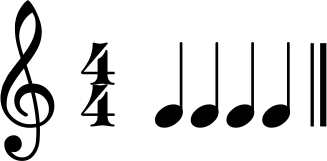
\includegraphics[scale=0.3]{img/discuss1}\\
\hline
\end{tabular}
}
}

\subfloat[Parser interpretation.]{
\label{fig:rests:b}
\parbox{0.5\linewidth}{
\Tree
[ .{$\frac{1}{1}$} [ .{$\frac{1}{2}$} [ .{$\frac{1}{4}$} [ .$*$ ] [ .$\bullet$ ] ] [ .{$\frac{1}{4}$} [ .$\bullet$ ] [ .$\bullet$ ] ] ] [ .$\bullet$ ] ] 
}
}
\subfloat[]{
\parbox{0.5\linewidth}{
\begin{tabular}{| l  >{\centering\arraybackslash}m{2in} |}
\hline 
A & 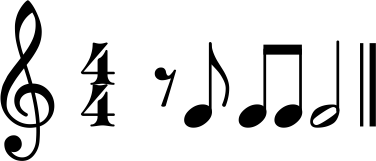
\includegraphics[scale=0.3]{img/discuss2}\\
B & 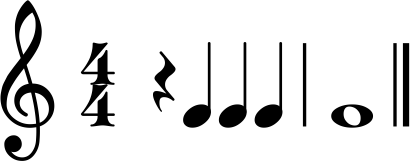
\includegraphics[scale=0.3]{img/discuss3}\\
\hline
\end{tabular}
}
}

\parbox{0.4\linewidth}{
\subfloat[A representation that includes rests.]{
\label{fig:rests:c}
\Tree
[ .{$\frac{1}{1}$} [ .{$\frac{1}{2}$} [ .{$\frac{1}{4}$} [ .$*$ ] [ .$\bullet$ ] ] [ .{$\frac{1}{4}$} [ .$\bullet$ ] [ .$\bullet$ ] ] ] [ .{$\frac{1}{2}$} [ .{$\frac{1}{4}$} [ .$\bullet$ ] [ .Rest ] ] [ .Rest ] ] ]
}
}
\subfloat[]{
\parbox{0.5\linewidth}{
\begin{tabular}{| l  >{\centering\arraybackslash}m{2in} |}
\hline 
A & 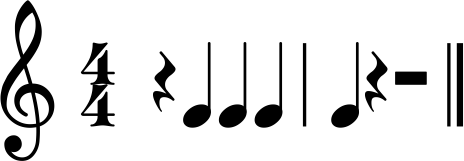
\includegraphics[scale=0.3]{img/discuss4}\\
\hline
\end{tabular}
}
}
\caption{An example of why rests are desirable to correctly represent the last note.}
\label{fig:rests}
\end{figure}

%\chapter{Conclusion}
\label{sec:conclusion}

% Tempo invariant approach
% Tempo and time signature is/can be detected.
% Detection of tactus, meter and transcription integrated in one approach
% Rests are needed
% More data is needed for expression
%\section{Future Work}
\label{sec:futurework}

\appendix
\include{sections/appendix}

\bibliographystyle{plainnat}
\bibliography{refs}

\end{document}